\chapter{L'Intelligence Ambiante au sein des habitats intelligents}
\label{chap:2}

\section{Introduction}

Dans le chapitre précédent, la reconnaissance d'activité a été définie et son application concrète au sein d'environnements intelligents a été brièvement abordée. Néanmoins, avant d'entrer plus en détail sur le fonctionnement du processus de la reconnaissance d'activité, il convient d'étudier les différents types d'environnements dans lesquels elle est appliquée. Ainsi, ce chapitre présente, dans un premier temps, l'état de l'art des différents types d'architectures existantes pour enfin, proposer une étude détaillée du processus de la reconnaissance d'activités. Cette dernière partie présentera notamment l'ensemble des étapes nécessaires pour y parvenir ainsi que les différents algorithmes utilisés.

\section{Les habitats intelligents existants}

Dans la dernière décennie, plusieurs implémentations d'habitats intelligents, visant à mettre en pratique le concept de reconnaissance d'activités multicouche tel que présenté par \cite{Roy2013}, ont émergé \citep{DJCook2003, Helal2005, Giroux2009, Cook2013, Bouchard2014, Lago2017}. Néanmoins, en l'absence de toute spécification formelle d'une architecture optimale pour ces habitats, chacune des applications proposées demeurent différentes malgré leur motivation commune. Puisque l'un des objectifs de cette thèse est de proposer une meilleure intégration des \textit{wearable devices} au sein des habitats intelligents\textemdash il convient d'identifier les réelles différences entre ces architectures afin d'en extraire leurs avantages et leurs inconvénients. Pour ce faire, cette première partie se découpe en trois sous-sections qui correspondent chacune à un type d'implémentation parmi les plus avancées dans le domaine soit, les architectures industrielles avec le \acs{LIARA} \citep{Bouchard2014} et le \acs{DOMUS} \citep{Giroux2009}, les architectures basées composants avec MavHome \citep{DJCook2003}, Gator-Tech \citep{Helal2005} et Amiqual4home \citep{Lago2017} et enfin CASAS \citep{Cook2013}, l'habitat intelligent qui repose sur un réseau maillé ZigBee. Cependant, cette thèse ne tient pas compte des habitats intelligents qui reposent sur l'utilisation de technologies considérées trop intrusives pour reconnaître les activités de leurs résidents, comme les caméras ou les microphones \citep{Brumitt2000, Vacher2011}.

\subsection{Héritage Industriel}

Le \acs{LIARA} \citep{Bouchard2014} et le Laboratoire \acs{DOMUS} \citep{Giroux2009} sont deux environnements académiques de recherche pour la reconnaissance d'activités. Ces deux laboratoires disposent d'habitats intelligents qui reposent sur des technologies héritées du milieu industriel. Comme illustré à la figure \ref{fig:archi_liara_domus}, leur architecture s'articule essentiellement autour d'une entité de calcul centrale (le serveur) ainsi qu'un automate industriel qui permet de récupérer les valeurs des différents capteurs qui sont divisés en îlots. Ces valeurs sont ensuite enregistrées dans une base de données de type relationnelle. Ainsi, les couches supérieures de la reconnaissance d'activités peuvent être réalisées sur le serveur par le biais d'une unique interface.

\begin{figure}[t]
	\centering
	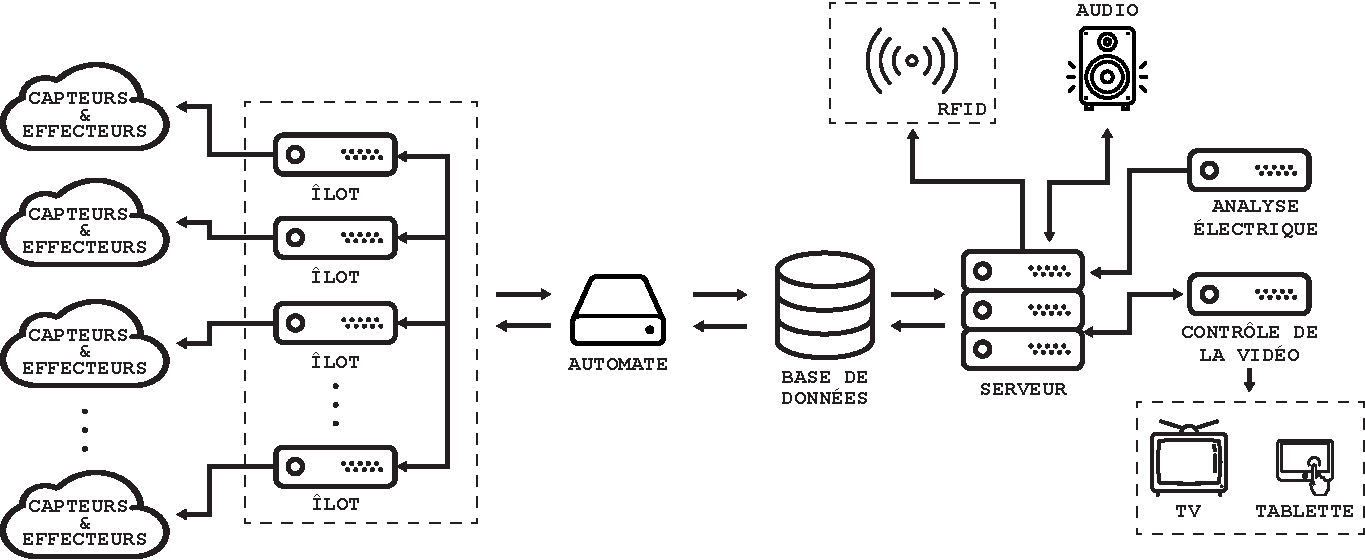
\includegraphics[width=\linewidth]{chapter2/archi_liara_domus.pdf}
	\caption{Architecture du \acs{LIARA} et du laboratoire \acs{DOMUS}.}
	\label{fig:archi_liara_domus}
\end{figure}

Le principal avantage d'une telle architecture concerne l'exploitation de matériel industriel directement. En effet, ce dernier étant conçu pour fonctionner sans interruption dans des environnements difficiles comme des usines, il demeure extrêmement robuste et fiable sur le long terme. Cela permet donc de garantir la qualité de fabrication pour l'habitat intelligent. Aussi, le choix d'une architecture centralisée favorise un accès simplifié aux données de l'habitat. La couche matérielle est abstraite pour les différents programmes de reconnaissance et d'assistance qui peuvent alors interroger directement la base de données.

Malgré ces avantages, une architecture comme celle du \acs{LIARA} et du laboratoire \acs{DOMUS} présentent des inconvénients majeurs. Le premier concerne le coût global. En effet, \cite{Plantevin2018a} a évalué le prix de ces habitats à 13 500 dollars US sans compter les capteurs, les effecteurs, l'installation et le support. Un investissement de cette ampleur est donc conséquent pour les personnes en perte d'autonomie, car dans une grande majorité, ceux-ci vivent dans des conditions financières précaires, et ce, malgré la prise en charge de certains frais par leur régime d'assurance \citep{AlzheimersAssociation2018}. De plus, bien que le matériel industriel soit un gage de qualité de l'habitat, il n'est pas impossible qu'une panne survienne, par exemple la perte d'un îlot, de l'automate ou du serveur. De ce fait, puisque l'architecture est centralisée, le fonctionnement de l'habitat peut être partiellement ou totalement altéré. Dans le pire des cas, l'assistance au résident devient donc impossible et des situations dangereuses pour sa sécurité peuvent survenir. Finalement, une architecture monolithique telle que celle-ci ne facilite pas l'intégration de nouveaux capteurs qui doivent être ajoutés manuellement dans le système. De plus, l'intégration de capteurs qui ne peuvent être reliés par câble aux îlots de l'habitat demeure extrêmement complexe \citep{Plantevin2018a}. Il apparaît donc clairement que l'évolutivité de l'architecture ainsi que l'utilisation de \textit{wearable devices} n'ont pas été pris en compte lors de la conception de cette architecture.

\subsection{Open Services Gateway initiative}

Pour répondre à la problématique de l'évolutivité, des architectures basées composant ont été développées. Le premier exemple d'habitat intelligent exploitant ce type d'architecture est MavHome \citep{DJCook2003}. Cette dernière repose sur une interface \ac{CORBA}\footnote{\url{www.corba.org}} permettant la liaison entre les différents composants logiciels et le contrôleur électrique des appareils présents dans l'habitat. Cependant, en raison de la complexité des contraintes imposées par ce standard, des solutions plus récentes comme Gator-Tech \citep{Helal2005}, Amiqual4home \citep{Lago2017} ou encore les initiatives proposées par \cite{Novak2011} et \cite{Cheng2012} ont préféré l'emploi de la technologie \ac{OSGi}\footnote{\url{www.osgi.org/developer/architecture}}. Tous ces habitats partagent des caractéristiques identiques. Par conséquent, seuls les cas de Gator-Tech et d'Amiqual4home seront détaillés dans cette section, car ils reviennent fréquemment dans la littérature.

L'habitat Gator-Tech a pour objectif de répondre à une problématique des habitats de type industriel, à savoir la simplification du processus d'intégration de nouveaux capteurs. Pour ce faire, son architecture repose essentiellement sur la technologie \acs{OSGi}. Comme illustré par la figure \ref{fig:archi_gator_tech}, chaque capteur de l'habitat possède son propre pilote qui lui permet de communiquer avec l'intégralité du système. Ce pilote est stocké dans une mémoire morte dans le but de conserver les données, même lorsque le matériel n'est pas alimenté. Ainsi, lors de la mise en fonction d'un capteur, celui-ci s'enregistre de manière autonome auprès d'une définition de service. Cette dernière va alors servir de couche d'abstraction pour la création de services de base qui peuvent soit permettre de consommer des données fortement abstraites, soit être combinés afin d'obtenir un service composite. Un service de base peut, par exemple, renvoyer \textit{``la plaque de cuisson est chaude''} lorsque la sonde de température de la cuisinière donne une valeur supérieure à 50\textdegree{}C ; alors qu'un service composite peut, quant à lui, agréger tous les services basiques des capteurs \ac{RFID} pour localiser un résident dans l'habitat. De ce fait, il est possible de concevoir des programmes de reconnaissance et d'assistance sans jamais se préoccuper du protocole de communication des capteurs, ni du format dans lequel ils transmettent les données.

Ce même fonctionnement est utilisé par l'habitat intelligent Amiqual4home. Cet environnement s'appuie sur \ac{openHAB}\footnote{\url{www.openhab.org}}, un \textit{middleware open source} dédié aux habitats intelligents, qui s'appuie sur un environnement \acs{OSGi} ainsi que sur le \textit{framework} Eclipse SmartHome\footnote{\url{www.eclipse.org/smarthome}} spécifiquement conçu pour fonctionner dans cet environnement. Ainsi, comme illustré par la figure \ref{fig:archi_amiqual4home}, \acs{openHAB} permet de créer une couche d'abstraction autour des couches service, connaissance et logicielle visibles sur la figure \ref{fig:archi_gator_tech}.

Le principal avantage de ce type d'architectures est qu'elles supportent parfaitement la mise à l'échelle de l'environnement dans le cas d'ajouts ou de remplacements de capteurs. Il semble également que l'intégration de \textit{wearable devices} soit possible, sans effort particulier, grâce à la flexibilité offerte par les architectures basées composants. De plus, l'exploitation de données fortement abstraites facilite le développement de programmes de reconnaissance et d'assistance, puisqu'un raisonnement sur ce type de données demeure plus simple que d'exploiter les données brutes directement \citep{Helal2005}. Enfin, il est possible que le coût d'un tel habitat soit considérablement réduit en comparaison à un habitat basé sur une architecture industrielle. En effet, dans le cas de Gator-Tech, son architecture requiert toujours un serveur central. Néanmoins, elle n'implique pas l'utilisation d'un automate ou d'îlots, et les capteurs utilisés au sein de cet environnement sont basés sur des plateformes à faible coût \citep{Helal2005}. Cependant, tout comme pour les habitats de type industriels, Gator-Tech et les autres architectures basées composant souffrent du même inconvénient majeur, c'est-à-dire, le recourt à un serveur central comme seule unité de calcul. Dans le cas présent, ce dernier provoque la création d'un goulot d'étranglement. En effet, un large flux de données qui transitent par le serveur peut entraîner un ralentissement de celui-ci. Il devient alors surchargé et l'assistance pour le résident n'est plus réalisée convenablement.

\begin{figure}[H]
	\centering
	\subfloat[Gator-Tech]{
		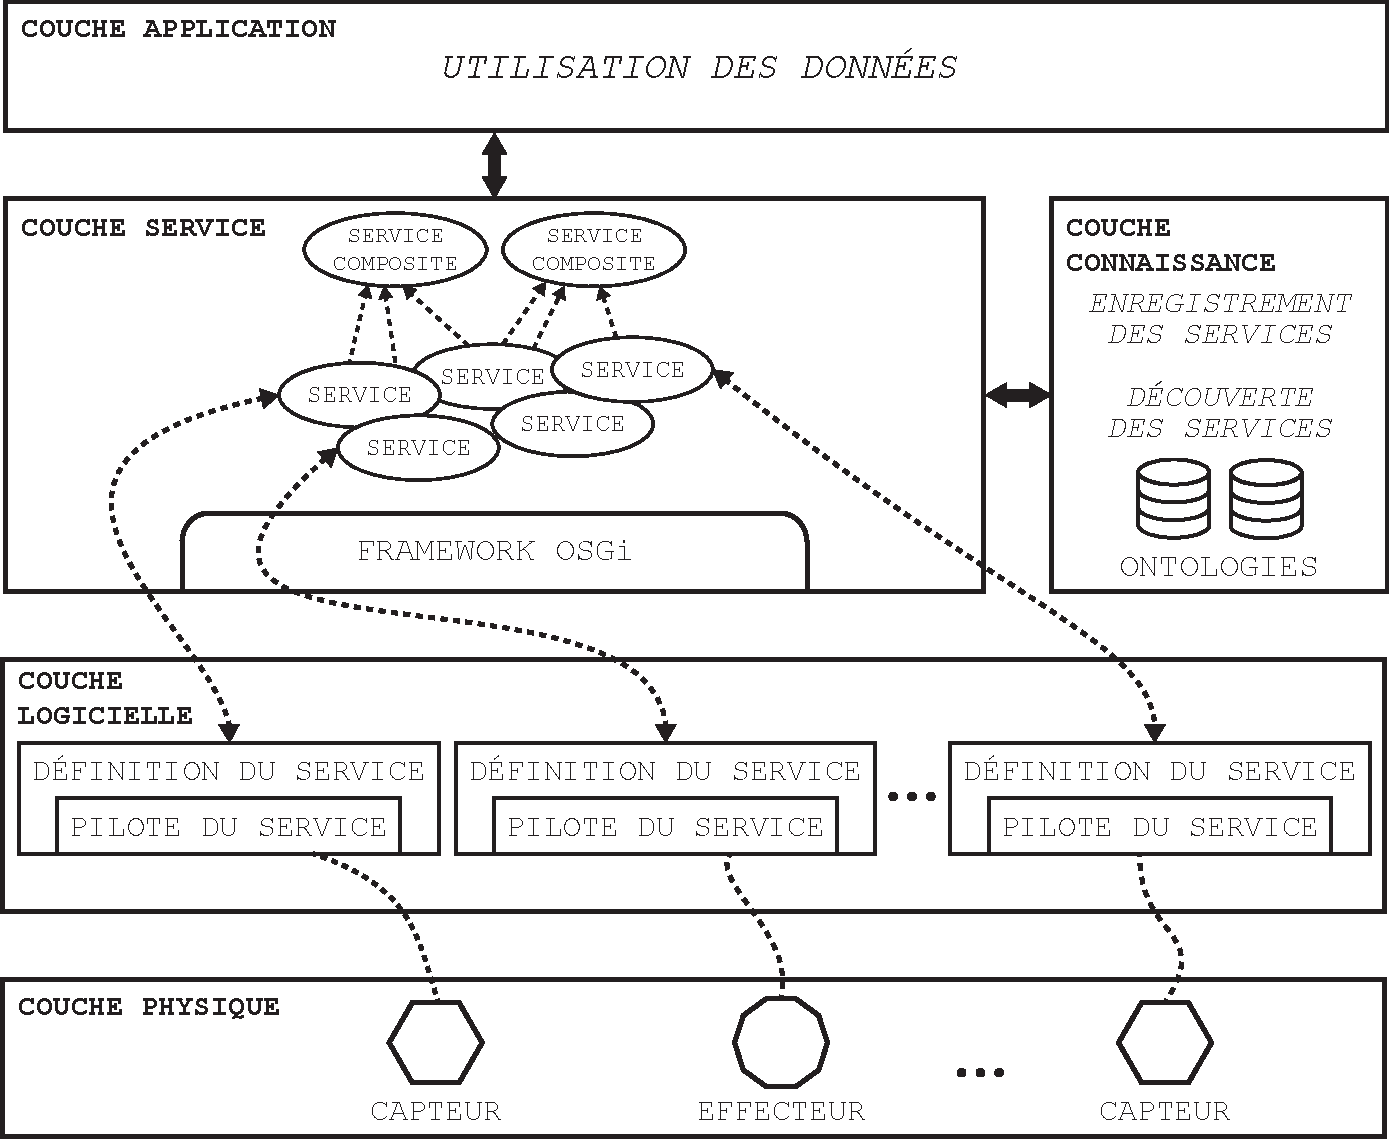
\includegraphics[width=.8\linewidth]{chapter2/archi_gator_tech.pdf}
		\label{fig:archi_gator_tech}
	}
	\\[20pt]
	\subfloat[Amiqual4home]{
		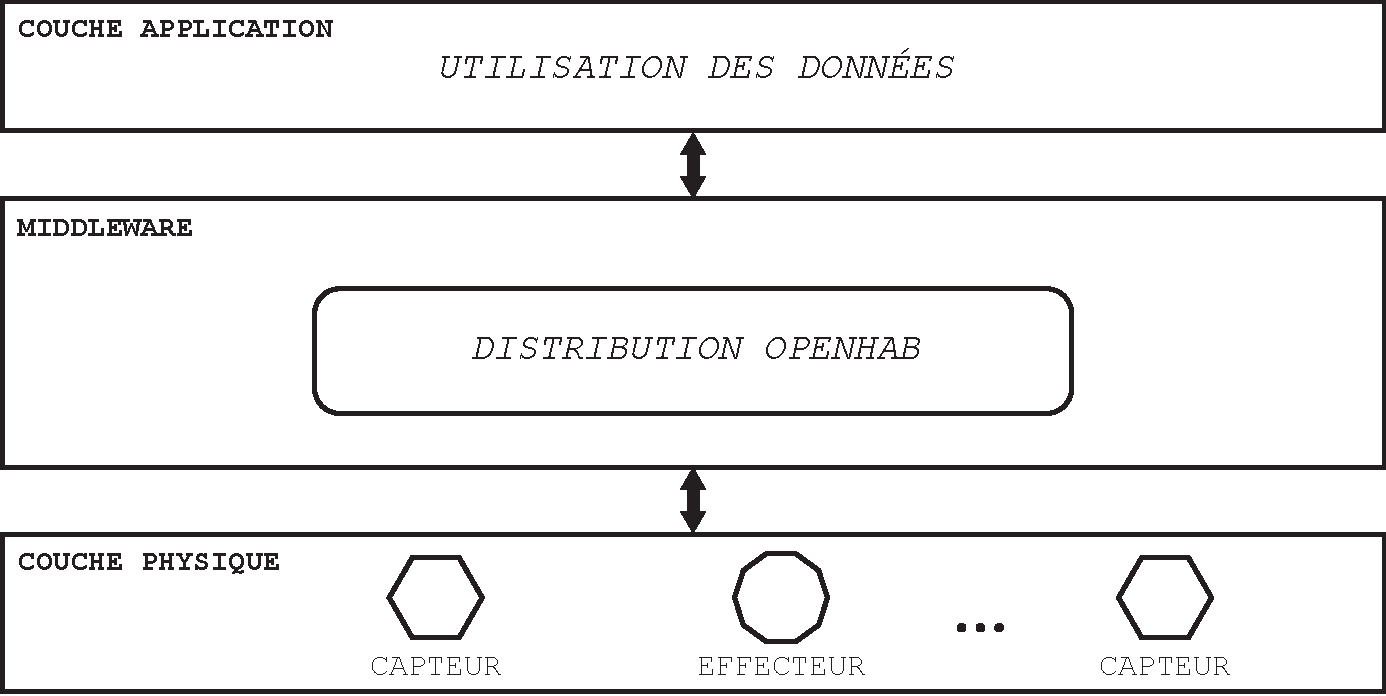
\includegraphics[width=.8\linewidth]{chapter2/archi_amiqual4home.pdf}
		\label{fig:archi_amiqual4home}
	}
	\caption{Architectures des habitats intelligents Gator-Tech et Amiqual4home}
\end{figure}

\subsection{Réseau Maillé}

Grâce aux récentes avancées des technologies de communication sans-fil, de nouveaux types d'habitats intelligents ont émergés. Ainsi, des initiatives telles que CASAS \citep{Cook2013}, ou encore celles proposées par \cite{Zhihua2016} et \cite{Zhenyu2011} ont été proposées. Toutes s'articulent autour d'un réseau maillé ZigBee, une technologie de communication sans fil qui sera expliqué plus en détail dans la figure \ref{subec:com_zigbee}. Bien qu'ils admettent des différences, ces trois habitats demeurent sensiblement identiques dans la conception de l'architecture qu'ils proposent. De ce fait, cette section ne traite exclusivement du cas de CASAS, puisque celui-ci reste le plus connus d'entre eux. En introduisant CASAS, \cite{Cook2013} voulaient principalement résoudre le problème du coût que représentent les habitats intelligents, mais également en faciliter leur installation. C'est ainsi que le concept d'habitat intelligent en boîte est né. Comme montré par la figure \ref{fig:archi_casas}, l'architecture de CASAS se décompose en quatre composants principaux. Tout d'abord, il y a la couche physique qui contient le réseau maillé ZigBee. Dans le cas de cet habitat, il s'agit d'une topologie de réseau sans-fil où tous les n\oe{}uds, c'est-à-dire les capteurs et les effecteurs, sont connectés pair à pair et collaborent pour s'échanger des données. Le réseau maillé communique ensuite avec un service de messagerie au travers un pont ZigBee. Ce dernier a pour but de transformer les données des capteurs en messages \ac{XMPP} de plus haut niveau. Le service de messagerie étant de type \textit{publish/subscribe}, il offre alors la possibilité à d'autres services de s'y connecter. C'est notamment le cas du service d'archivage. Ce dernier récupère, par l'intermédiaire du pont scribe, certains évènements qui se produisent dans l'habitat afin de les enregistrer dans une base de données d'archives. Finalement, les applications de reconnaissance et d'assistance exploitent les données du \textit{middleware} en les récupérant \textit{via} le pont applicatif.

\begin{figure}[H]
	\centering
	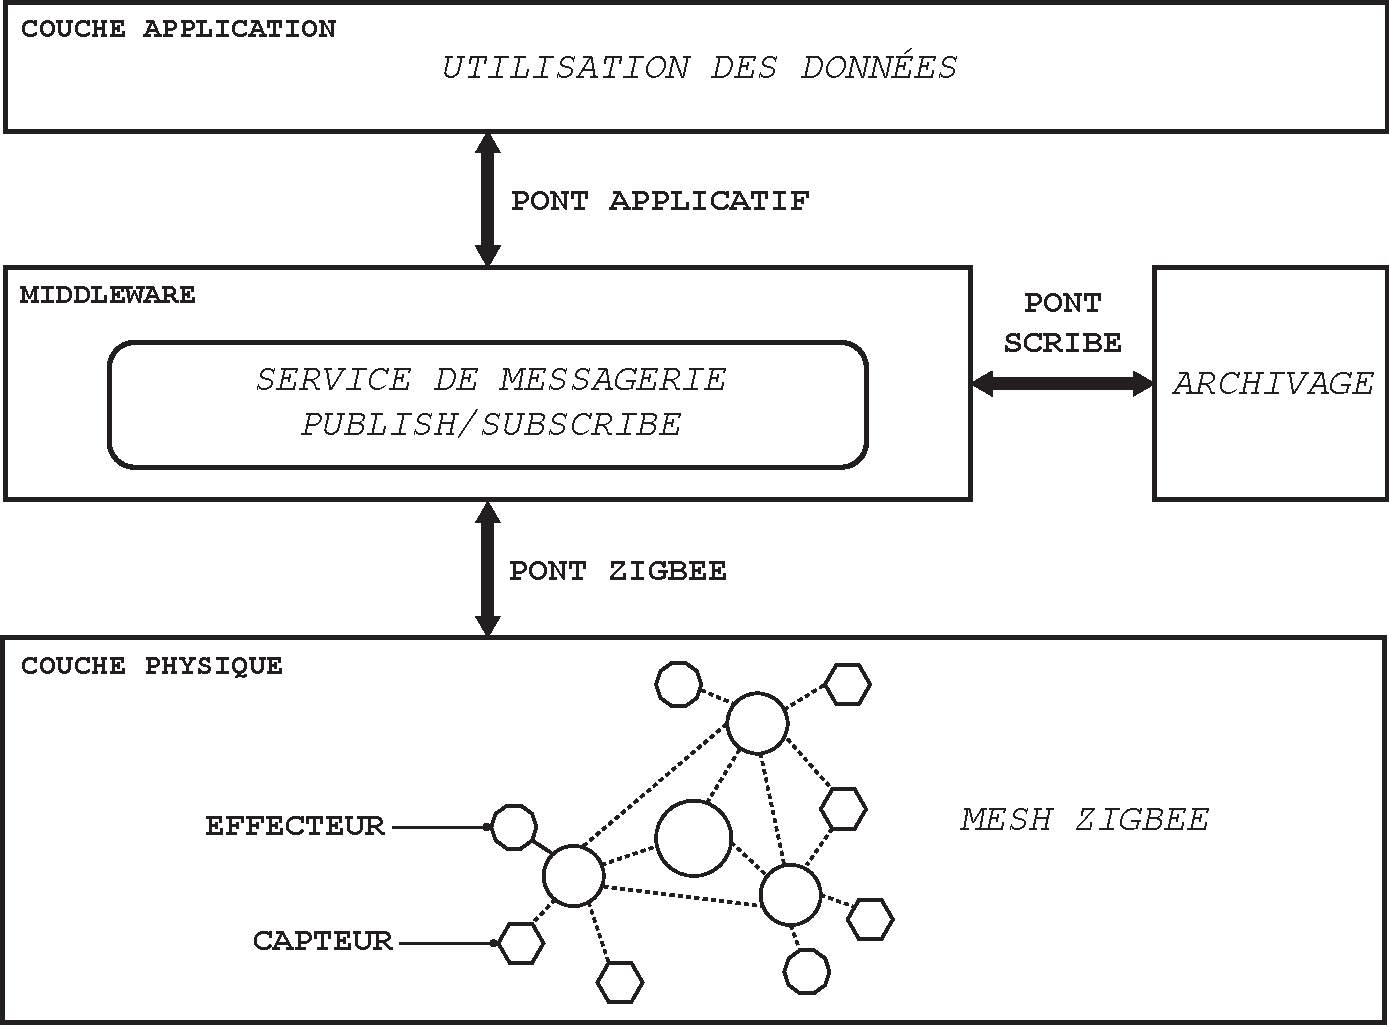
\includegraphics[width=.8\linewidth]{chapter2/archi_casas.pdf}
	\caption{Architecture de l'habitat intelligent CASAS.}
	\label{fig:archi_casas}
\end{figure}

Les habitats intelligents basés sur les réseaux maillés ZigBee sont des solutions réellement moins onéreuses que les autres types d'architectures d'habitats. En effet, \cite{Cook2013} rapportent un coût total estimé à 2 765 dollars US, soit presque cinq fois moins qu'un habitat industriel. Par ailleurs, puisque les habitats basés sur un réseaux maillé reposent tous sur la technologie de communication sans-fil ZigBee, il semble relativement aisé d'y ajouter de nouveaux capteurs et notamment d'y intégrer des \textit{wearable devices}. Cependant, l'inconvénient majeur du protocole ZigBee est que les signaux ne sont pas directement compatibles avec des systèmes évolués tels que les ordinateurs ou les téléphones intelligents. De plus, tous les \textit{wearable devices} ne disposent pas toujours d'une connectivité ZigBee. En effet, la grande majorité d'entre eux ont plutôt adopté la technologie \ac{BLE} \citep{Martin2014}, qui est également devenue compatible avec la topologie réseau maillé récemment \citep{Bluetooth2017}. Enfin, les architectures comme CASAS souffrent elles aussi de plusieurs points de défaillances qui remettent en question leur fiabilité quant à l'assistance rigoureuse que doivent recevoir les habitants d'une maison intelligente (\textit{p. ex.} les ponts entre les différentes couches).

Il apparaît donc clairement qu'une architecture adaptative pour l'intégration des \textit{wearable devices} est nécessaire. Bien que les architectures basées sur un réseau maillé constituent un premier pas en ce sens, la variété des technologies de communication et des protocoles qu'elles peuvent exploiter n'est pas encore pleinement prise en compte dans leur conception.

\subsection{Transducteurs Intelligents Distribués}

Le principal inconvénient partagé par toutes les architectures de maisons intelligentes identifié dans les sections précédentes réside dans la centralisation de leur conception. En effet, chacune d'entre elles possède au moins un point de défaillance. Ceux-ci peuvent conduire à un dysfonctionnement partiel ou total du processus de reconnaissance d'activités qui est effectué au sein de ces habitats et ainsi potentiellement compromettre la sécurité de leurs résidents. Toutefois, cette problématique en particulier a été traitée il y a plusieurs années, dans différents domaines de l'informatique, tels que le calcul distribué, à l'aide de mécanismes de redondance et de partitionnement de données (\textit{clustering}) \citep{Dikaiakos2009,Zaharia2010,JafarnejadGhomi2017}.


\begin{figure}[ht!]
	\centering
	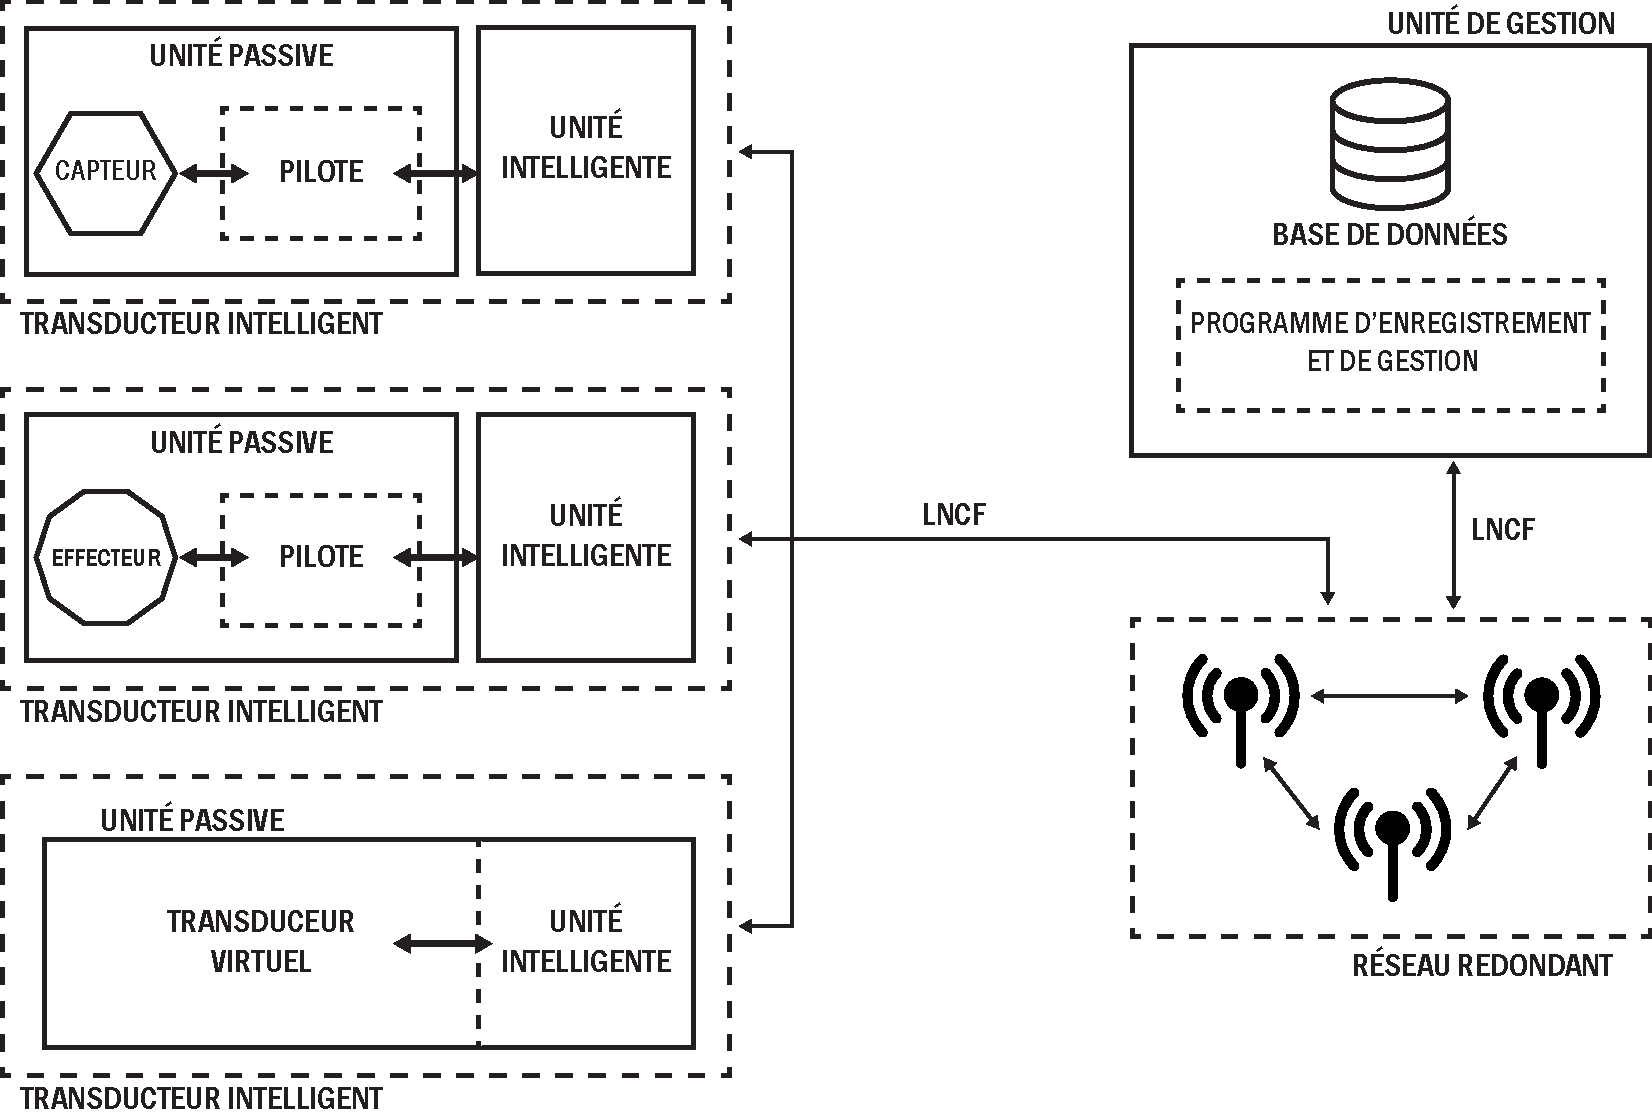
\includegraphics[width=.8\linewidth]{chapter2/archi_smart_transd.pdf}
	\caption{Architecture qui repose sur l'utilisation de transducteurs intelligents.}
	\label{fig:archi_smart_transd}
\end{figure}

Dans cette optique, \cite{Plantevin2018} ont plus récemment proposé une architecture de maison intelligente distribuée qui n'inclue
pas de point de défaillance critique. Pour ce faire, il ont suggéré la mise en place de transducteurs intelligents, définis selon la norme IEEE 1451.4 \citep{InstituteofElectricalandElectronicsEngineers1999}. Comme illustré en figure \ref{fig:archi_smart_transd} les transducteurs intelligents peuvent être de deux types différents. Les transducteurs physiques et les transducteurs virtuels, chacun étant composé de deux unités distinctes, l'unité passive et l'unité intelligente. Qu'elle soit matérielle ou logicielle, l'unité passive sert à produire des données de haut niveau à partir d'un ensemble d'évènements de bas niveau qui se produisent dans l'environnement extérieur. Par ailleurs, l'unité intelligente, quant à elle, représente l'entité de calcul principale qui fait qu'un transducer demeure autonome. En effet, son rôle est de communiquer avec le reste de l'environnent et d'exécuter les applications nécessaire pour réaliser le processus de reconnaissance d'activités grâce aux données acquises auprès de l'unité passive. La communication entre ces deux unités est réalisée soit \textit{via} un lien série pour les tranduceurs matériels, soit par le biais d'une communication de type \textit{publish/subscribe} basée sur ZeroMQ\footnote{\url{https://zeromq.org}} pour les transducteurs virtuels. Puisque cette architecture repose sur un très grand nombre de transducteurs intelligents, ceux-ci sont tous interconnectés par un réseau sans fil redondant qui leur permet de communiquer entre eux par l'intermédiaire du protocole \ac{LNCF}\textemdash un protocole également introduit par \cite{Plantevin2017}. Enfin, tous les transducteurs doivent s'enregistrer auprès d'une éntité centrale afin de récupérer le pilote ainsi qu'un fichier d'instructions pour leur permettre fonctionner de manière adéquat. Cette opération est effectuée une seule fois, lors du premier demarrage des transducteurs. De ce fait, bien que cette unité de gestion soit nécessaire pour l'installation de nouveaux transducteurs, son rôle est, par la suite, d'assurer le suivis des transducteurs qui composent l'architecture et d'emettre des alertes dans le cas où un transducteur serait en panne.

L'avantage principal de cette récente implémentation d'architecture est qu'elle demeure évolutive vis-à-vis du matériel, c'est-à-dire que la mise en place de nouveaux capteurs y est à la fois possible et facilitée. De plus, puisque l'objectif principal était de supprimer les points de défaillance, cette architecture offre un excellent niveau de fiabilité, car le dysfonctionnement d'un transducteur en particulier n'affecte pas le système dans son intégralité. Il est alors toujours possible de réaliser le processus de reconnaissance d'activité pour offrir l'assistance requise aux résidents de l'habitat. Bien que l'unité de gestion demeure toujours un point central dans la conception de cette architecture, les auteurs ont mentionné que cette entité peut être hébergée dans le \textit{cloud}. Ceci afin de garantir la fiabilité de sa disponibilité en cas de défaillance. De plus, puisque cette unité est indispensable uniquement lors de la première mise en place de l'architecture ou pour ajouter de nouveaux transducteurs, le bon fonctionnement de l'habitat intelligent ne sera pas compromis en cas de panne. En ce sens, il reste possible de réaliser une opération de maintenance sans mettre en danger les habitants de la maison intelligente. Néanmoins, la prise en charge de l'hétérogénéité des composants logiciels qui constituent le processus de la reconnaissance d'activités semble avoir été mise de côté dans la conception de cette architecture.

\section{Le processus d'apprentissage pour la reconnaissance des activités}

\begin{figure}[b!]
	\centering
	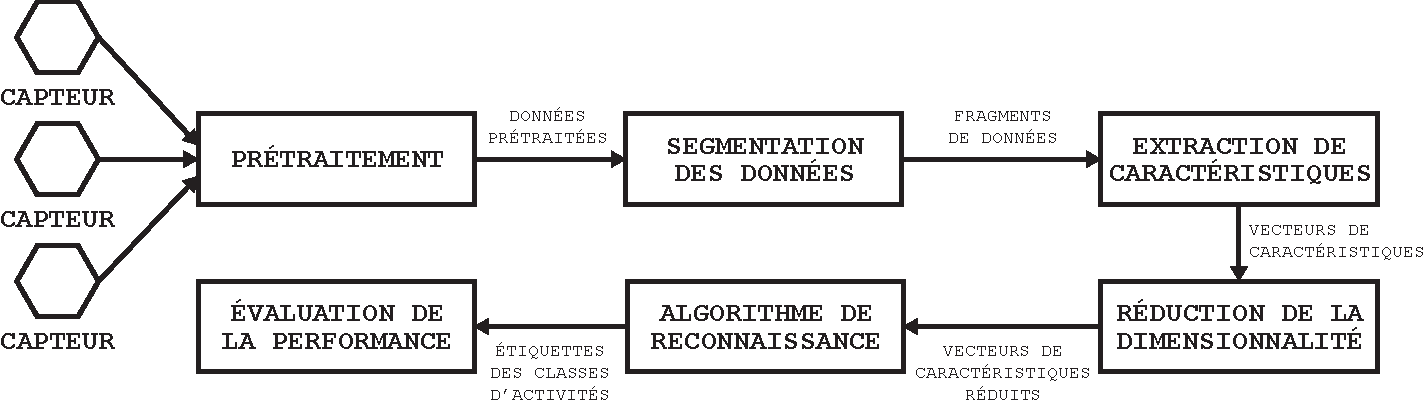
\includegraphics[width=\linewidth]{chapter2/ar_process.pdf}
	\caption{Processus d'apprentissage pour la reconnaissance d'activités.}
	\label{fig:ar_process}
\end{figure}

Le processus d'apprentissage pour la reconnaissance d'activités est un ensemble d'étapes qu'il est généralement possible de réaliser pour reconnaître des activités. Tel qu'illustré par la figure \ref{fig:ar_process}, ce processus requiert des données initiales fournies par les capteurs ambiants ou portables. Celles-ci n'ont alors été soumises à aucun traitement en particulier, ce sont donc des données brutes. Principalement en fonction de la condition des capteurs et de la transmission des valeurs, les données obtenues peuvent se retrouver altérées. Afin d'améliorer leur qualité, il est donc possible, dans un second temps, d'effectuer une étape de prétraitement. Ensuite, puisque les données renvoyées représentent un signal ayant une longueur potentiellement infinie, il est impératif de segmenter ce dernier en plusieurs fragments, sur chacun desquels, des propriétés discriminantes sont calculées. L'ensemble de celles-ci, une fois extraites, constitue alors une abstraction du fragment traité. Le signal fragmenté est donc réduit à un unique vecteur de caractéristiques pour chaque segment. Dans certains cas, il peut s'avérer que celui-ci contienne un nombre de propriétés suffisant pour impacter négativement la performance de la reconnaissance\textemdash auquel cas, une étape supplémentaire pour réduire la dimensionnalité du vecteur est requise. Cet ensemble de données est ensuite utilisé comme entrée d'un algorithme d'apprentissage qui, pour chacun des vecteurs réduits, retournera les noms des classes associées aux activités à reconnaître. Finalement, la dernière étape du processus consiste en une évaluation de la performance de la reconnaissance.

\subsection{Les étapes préliminaires}
\label{sec:prel_steps}

Avant d'être en mesure d'utiliser les algorithmes d'apprentissage, il est nécessaire que les données brutes issues des capteurs passent par un ensemble d'étapes préliminaires pour être transformées en caractéristiques discriminantes. Ainsi, cette section présente les méthodes les plus utilisées en ce qui concerne le prétraitement et la segmentation des données, mais également l'extraction de caractéristiques et la réduction du nombre qui en est produit, c'est-à-dire la réduction de la dimensionnalité.

\subsubsection{Prétraitement des données}

Le prétraitement des données est la première étape du processus d'apprentissage pour la reconnaissance d'activités. En effet, après l'acquisition des valeurs renvoyées, autant par les capteurs ambiants que les capteurs portables présents au sein d'un environnement intelligent, plusieurs facteurs peuvent influer sur la qualité de ces données. Par exemple, un mauvais fonctionnement du matériel ou un problème de transmission comme une latence réseau peuvent entraîner l'acquisition de données incohérentes, erronées ou encore partiellement manquantes. L'objectif de cette étape sont donc d'améliorer les données récoltées en réduisant le bruit, ou en filtrant les éléments nuisibles, tout en essayant de conserver les caractéristiques dynamiques essentielles du signal.

Dans le cas où les données comprendraient des valeurs partiellement manquantes, plusieurs méthodes peuvent être employées pour pallier cette perte. Dans un premier temps, il est tout simplement possible d'ignorer les données incriminées. Néanmoins, cette méthode n'est pas pertinente lorsque l'absence d'information est très élevée. De ce fait, il est possible de remplacer les valeurs manquantes pour un attribut donné grâce à une estimation qui peut être déterminée selon deux procédés différents. Le premier consiste à calculer la moyenne de toutes les valeurs non manquantes pour l'attribut en question. La seconde méthode implique que les données soient étiquetées et consiste à remplacer la valeur manquante d'un attribut par la moyenne des valeurs présentes qui appartiennent à la même classe celui-ci.

De plus, il est admis que les capteurs \ac{RFID} et les accéléromètres sont connus pour être les deux types de capteurs (ambiant et portable) les plus sujets au bruit. Or, de nombreux travaux se basent sur l'exploitation de ceux-ci dans le but de reconnaître des activités \citep{Ravi2005, Stikic2008, Buettner2009, Khan2011, Mannini2017}. De ce fait, \cite{Wang2011} ont comparé quatre filtres différents ayant pour but de réduire le bruit dans les données générées par un accéléromètre, soit : un filtre médian \citep{Huang1979}, un filtre passe-bas de type \textit{Butterworth} \citep{Butterworth1930}, une transformée en ondelettes discrète spécifique (\ac{DWPD}) \citep{Mallat1989} et un filtre de Kalman \citep{Welch2006}, où ce dernier s'est révélé comme le plus efficace. \cite{Abreu2014} ont, quant à eux, montré que le filtre de Kalman était également le plus performant pour réduire le bruit présent dans le leur système de localisation intérieure basé sur des capteurs \acs{RFID}.

\subsubsection{Segmentation des données}
%%%
% Dans le processus d'apprentissage, la segmentation des données peut intervenir, soit après la première phase de prétraitement, soit directement sur les données brutes si celles-ci ne sont pas altérées. Cette opération consiste à découper un signal donné $X$ en plusieurs fragments plus petits $x_i$. Chaque segment $x_i = (T_1, T_2)$ est alors délimité par un temps de départ $T_1$ et un temps d'arrivée $T_2$. Le signal est donc morcelé en une séquence de segments tel que,

% \begin{equation}
%     X = \left\{x_n\right\}, \quad n \in \mathbb{N} .
% \end{equation}

% \noindent Du point de vue du traitement de signal, cette opération est appelée le fenêtrage. Ainsi, il est possible d'observer le signal d'origine $x\left(t\right)$ de longueur théoriquement infinie, sur une durée finie $T$ en le multipliant par une fonction fenêtre d'observation $w\left(t\right)$ tel que,

Dans le processus d'apprentissage, la segmentation des données peut intervenir, soit après la première phase de prétraitement, soit directement sur les données brutes si celles-ci ne sont pas altérées. Cette opération consiste à découper un signal donné en plusieurs fragments plus petits. En d'autres termes, le signal est morcelé en une séquence de segments qui sont délimités par un temps de départ et un temps d'arrivée. Du point de vue du traitement de signal, cette opération est appelée le fenêtrage. Ainsi, il est possible d'observer le signal d'origine $x\left(t\right)$ de longueur théoriquement infinie, sur une durée finie $T$ en le multipliant par une fonction fenêtre d'observation $w\left(t\right)$ tel que,

\begin{equation}
    x_w\left(t\right) = x\left(t\right)w\left(t\right), \quad 0 \leq t \leq T - 1.
\end{equation}

En ce qui concerne la reconnaissance d'activités, il est possible de regrouper les techniques de segmentation en trois groupes distincts : la segmentation basée sur les activités, la segmentation basée sur des évènements et la segmentation par fenêtre glissante \citep{Banos2014}.

La segmentation basée sur les activités revient à partitionner le signal selon la détection d'un changement significatif correspondant à une activité. Un tel découpage peut-être réalisé grâce à l'analyse du domaine fréquentiel du signal ou de son énergie \citep{Sekine2000, Guenterberg2009}.

La segmentation basée sur les évènements exploite, quant à elle, un découpage du signal selon la manifestation d'évènements spécifiques. Par exemple, cette méthode est souvent utilisée dans la reconnaissance de la marche ou d'autres activités similaires comme courir, monter ou descendre des escaliers, \textit{etc. } Puisque ces activités sont cycliques et requièrent des actions inévitables (\textit{p. ex., } le contact du pied sur le sol), il est possible de segmenter le signal par l'analyse de l'accélération \citep{SantAnna2010}, mais également en exploitant d'autres types de données comme celles issues de capteurs de pression \citep{Crea2012}.

Enfin, la segmentation par fenêtre glissante peut se traduire comme étant la translation d'une fenêtre sur l'axe temporel du signal, où chaque déplacement de la fenêtre représente un segment. Une fenêtre est définie par une fonction mathématique, une taille ainsi qu'un pourcentage de superposition. En ce qui concerne ce dernier, si une fenêtre est définie comme ayant une taille de 100 secondes avec un pourcentage de superposition de 50\%, le premier intervalle sera $\left[0,100\right]$ tandis que le second sera $\left[50,150\right]$ et ainsi de suite. Parmi les fonctions de fenêtrage les plus fréquemment utilisées, il est possible de mentionner, la fenêtre de Hamming ($w(t)_H$), celle de Kaiser ($w(t)_K$), de Hann ($w(t)_N$) ou encore la fenêtre de Blackman ($w(t)_B$) respectivement exprimées par :

\begin{equation}
	\label{eq:hamming}
	w\left(t\right)_H = \left\{
	\begin{array}{ll}
		0.54-0.46\cos(\frac{2\pi t}{T-1}), & \mbox{si } 0 \leq t \leq T-1 \\
		0,								   & \mbox{sinon.}
	\end{array}
	\right.
\end{equation}

\begin{equation}
	\label{eq:kaiser}
	w\left(t\right)_K = \left\{
	\begin{array}{ll}
		\frac{I_0\left[\alpha\sqrt{1-(\frac{2t}{T-1}-1)^2}\,\right]}{I_0\left[\alpha\right]}, & \mbox{si } 0 \leq t \leq T-1 \\
		0,                                    & \mbox{sinon.}
	\end{array}
	\right.
\end{equation}

\begin{equation}
	\label{eq:hann}
	w\left(t\right)_N = \left\{
	\begin{array}{ll}
		0.5-0.5\cos(\frac{2\pi t}{T-1}), & \mbox{si } 0 \leq t \leq T-1 \\
		0, & \mbox{sinon.}
	\end{array}
	\right.
\end{equation}

\begin{equation}
	\label{eq:blackman}
	w\left(t\right)_B = \left\{
	\begin{array}{ll}
		0.42-0.5\cos(\frac{2\pi t}{T-1}) + 0.08\cos(\frac{4\pi t}{T-1}), & \mbox{si } 0 \leq t \leq T-1 \\
		0,                                    & \mbox{sinon.}
	\end{array}
	\right.
\end{equation}

\noindent où, $I_0 $ est la fonction de Bessel modifiée d’ordre zéro, $\alpha$ est le paramètre réel non nul caractérisant la forme de la fenêtre et $T$ est la taille de la fenêtre. Néanmoins, tous les paramètres impliqués dans le processus de la segmentation doivent être déterminés en fonction de la problématique, où l'objectif est de trouver le meilleur compromis entre la rapidité d'exécution et la performance de reconnaissance \citep{Banos2014}.

\subsubsection{Extraction de caractéristiques}

L'extraction de caractéristiques est une phase importante dans le processus d'apprentissage pour reconnaître des activités. L'objectif de cette opération consiste à produire un vecteur de caractéristiques discriminantes pour chaque fragment du signal généré, grâce à un certain nombre de fonctions mathématiques. Il existe deux principaux domaines auxquels appartiennent les différentes techniques d'extraction : le domaine temporel et le domaine fréquentiel \citep{Huynh2005, Figo2010, Cleland2013}. Les caractéristiques issues du domaine temporel demeurent les plus simples à obtenir. Il est notamment possible d'y retrouver des métriques statistiques comme la moyenne, la variance, l'écart type, l'asymétrie ou encore le kurtosis (la courbure) du signal, mais également des métriques dites \og enveloppe \fg comme la médiane, le minimum ou le maximum du signal. De plus, de nombreuses autres métriques temporelles peuvent être utilisées dans la reconnaissance d'activités, comme la corrélation entre deux signaux ou encore le \textit{zero crossing rate}\textemdash qui correspond au taux de changement de signe d'un signal. Les formules de l'asymétrie $S$, du kurtosis $K$ et de la corrélation $\rho$ de deux signaux $n \mbox{ et } n'$ sont respectivement données par :

\begin{equation}
	\label{eq:asymetrie}
	S \left(n\right) = \frac{N}{(N-1)(N-2)} \cdot \left(\sum_{i=1}^{N}{\frac{(n_i-\bar{n})^3}{\sigma_n^3}}\right)
\end{equation}

\begin{equation}
	\label{eq:kurtosis}
	K \left(n\right) = \frac{N(N+1)}{(N-1)(N-2)(N-3)} \cdot \left(\sum_{i=1}^{N}{\frac{(n_i-\bar{n})^4}{\sigma_n^4}-\frac{3(N-1)^2}{(N-2)(N-3)}}\right)
\end{equation}

\begin{equation}
	\label{eq:correlation}
	\rho\left(n, n^{\prime}\right) = \frac{cov\left(n, n^{\prime}\right)}{\sigma_n\cdot\sigma_{n^{\prime}}}
\end{equation}

\noindent où $N$ représente la taille d'un fragment du signal, $n_i$ est le $i^{\grave{e}me}$ élément du fragment, $\bar{n}$ est la valeur moyenne du fragment et $\sigma_n$ correspond à l'écart type du fragment.

D'autre part, afin d'exploiter des caractéristiques issues du domaine fréquentiel, il est nécessaire de réaliser un passage vers celui-ci, depuis le domaine temporel. Pour ce faire, il s'agit de calculer la transformée de Fourier discrète du signal. Dans la grande majorité des cas, c'est l'algorithme de la transformée de Fourier rapide (\acl{FFT} ou \acs{FFT}) qui est utilisé à cet effet \citep{Brigham1967}. Malgré sa popularité, il est également possible d'utiliser l'algorithme de Goertzel pour réaliser la transformation depuis le domaine temporel vers le domaine fréquentiel \citep{Sysel2012}. Dès lors, les caractéristiques fréquentielles qui peuvent être calculées sont, la composante continue (\textit{DC Component}), l'énergie spectrale $E$ et l'entropie $H$ tel que,

\begin{equation}
	\label{eq:energy_spec}
	E = \frac{1}{N}\cdot\left(\sum_{i=1}^{N}\mid{}n_i\mid\right)
\end{equation}

\begin{equation}
	\label{eq:entropy}
	H = - \sum_{i=1}^{N}{P_i}\ln P_i
\end{equation}

\noindent où $n$ représente un vecteur de nombres complexes de taille $N$ issu de la \acs{FFT}, $n_i$ est le $i^{\grave{e}me}$ élément du vecteur et $P_i$ est la probabilité de $n_i$ donnée par l'équation suivante :

\begin{equation}
	\label{eq:pi}
	 P_i = \frac{n_i}{N - E}
\end{equation}

En dernier lieu, \cite{Mitchell2013} ont proposé une méthode de reconnaissance d'activités qui repose sur l'analyse par ondelettes (\acl{DWT} ou \acs{DWT}). À l'inverse de la transformée de Fourier, cette technique permet d'obtenir des caractéristiques à la fois issues du domaine temporel et fréquentiel, par décomposition d'un signal en un ensemble de coefficients d'ondelettes.

\subsubsection{Réduction de la dimensionnalité}

La dernière étape préliminaire concerne la réduction de la dimensionnalité du vecteur de caractéristiques. Cette étape est importante dans la mesure où elle permet de sélectionner l'ensemble des valeurs qui seront conservées pour pallier le \textit{fléau de la dimension} \citep{Bellman1957}. Ce phénomène intervient lorsque la taille du vecteur de caractéristiques croît de manière conséquente. Les données peuvent alors se retrouver isolées et deviennent éparses, ce qui a pour effet de dégrader l'efficacité de la reconnaissance d'activités. Ainsi, en réduisant la dimensionnalité de ces données, l'objectif est de conserver les caractéristiques pertinentes tout en minimisant la perte d'information. Bien que ce processus doive permettre une meilleure reconnaissance, l'exploitation d'un plus petit vecteur peut également induire un traitement postérieur plus rapide.

Actuellement, il existe une quantité importante de techniques de réduction de dimensionnalité. Par conséquent, \cite{VanDerMaaten2009} ont proposé une taxonomie dans laquelle ils recensent l'ensemble des méthodes existantes. En premier lieu, il possible de retrouver des techniques de réduction de la dimensionnalité orientées vers la sélection de caractéristiques qui reposent sur des évaluations statistiques des données, comme la covariance ou l'entropie. L'avantage majeur de ces méthodes réside dans leur simplicité de mise en {\oe}uvre. D'autre part, bien qu'elle demeure une technique plus complexe, l'analyse par composantes principales (\acl{PCA} ou \acs{PCA}), a souvent été utilisée dans le domaine de la reconnaissance d'activités \citep{He2009, Altun2010, Chen2012, Leightley2013}. Elle permet, de transformer des caractéristiques qui sont initialement corrélées en de nouvelles caractéristiques décorrélées les unes des autres, les composantes principales.% Soit plus formellement, si $X=\left[x_1, x_2,\dotsc{},x_n\right]^T$ est un vecteur colonne de $n$ valeurs aléatoires ayant une moyenne nulle, l'objectif de cette méthode est de trouver une matrice orthogonale $V$ de taille $n\times k$ tel que $k \leq n$. Ainsi, la projection réduite $X'=VX$ de taille $k$ permet de conserver le plus de variances de $X$ que possible. La matrice $V$ définit la direction principale de la projection où ses composants sont calculés en utilisant la décomposition de celle-ci en éléments propres $C=E\Lambda E^T$ grâce à la matrice de covariance $C=E(XX^T)$. Les vecteurs propres $\Lambda=diag(\lambda_1, \lambda_2,\dotsc{}, \lambda_n)$ déterminent alors la variance des composantes principales. Finalement, les composantes principales $X'=\left[x^{\prime}_1, x^{\prime}_2,\dotsc{},x^{\prime}_n\right]$ sont obtenues par projection des données d'origines dans les directions principales $X'=E^TX$ \citep{Jolliffe2011}.

Le nombre de déclinaisons d'algorithmes de sélection de caractéristiques étant considérable, le choix quant à la méthode à adopter n'est pas trivial. En effet, celui-ci doit être fait en fonction de la problématique à traiter et l'algorithme adéquat est bien souvent déterminé de manière empirique. % Comme mentionné précédemment, plusieurs travaux dans le domaine de la reconnaissance d'activités ont exploité le \acs{PCA} et la performance de la reconnaissance obtenue était satisfaisante. Cependant, cette méthode ne peut pas être qualifiée comme étant la plus appropriée pour réduire la dimensionnalité des caractéristiques dans le cas d'un système de reconnaissance d'activités.

\subsection{Les algorithmes d'apprentissage}
\label{sec:algos}

Dans la section précédente, les différents processus de prétraitement ont été présentés. Ces étapes sont importantes puisqu'elles permettent de préparer les données afin de raffiner leur qualité avant qu'elles soient utilisées par un algorithme d'apprentissage. Ainsi, reconnaître avec précision les activités d'un résident est l'objectif principal des habitats intelligents afin qu'ils puissent recevoir une assistance la plus adaptée possible. Par conséquent, de nombreuses méthodes algorithmiques issues du domaine de l'intelligence artificielle ont été proposées pour parvenir à reconnaître des activités. Cette section présente donc l'ensemble des différentes méthodes parmi les plus utilisées dans ce domaine.

Les algorithmes d'apprentissage, également qualifiés d'algorithmes de reconnaissance ou de classification, peuvent être décomposés en deux grandes familles : les méthodes supervisées et non supervisées. Un algorithme est dit supervisé si les données recueillies sont divisées en deux sous-ensembles respectivement appelés ensemble d'entraînement et de validation où les deux ensembles de données contiennent des instances étiquetées avec la classe correspondante à une activité donnée. À l'inverse, les algorithmes non supervisés ne requièrent pas l'étiquetage des données. Cependant, il est également possible de rencontrer, à plus faible mesure, des techniques d'apprentissage semi-supervisées qui combinent l'utilisation de données étiquetées et non-étiquetées lors la phase d'entraînement \citep{Zhu2005, Chapelle2006}.

\subsubsection{Les algorithmes probabilistes}

Dans l'univers des algorithmes probabilistes, il est possible de retrouver méthodes bayésiennes qui constituent des méthodes supervisées probabilistes. Celles-ci s'articulent autour des réseaux bayésiens. Un réseau bayésien est définis par un graphe orienté acyclique dans lequel, chacun des n\oe{}uds (sommets) représente une variable aléatoire et chacune des arêtes correspond à la dépendance conditionnelle existante entre un ou plusieurs n\oe{}uds du graphe \citep{Heckerman1995}. Pour appliquer ce principe dans un système de reconnaissance d'activités, il s'agit de considérer que les n\oe{}uds du graphe correspondent aux actions ou aux activités et que les arêtes sont les liens qui lient des actions aux activités. Ces actions peuvent être conjointes à plusieurs activités. Par conséquent, si la probabilité de chaque activité ainsi que les probabilités conditionnelles des n\oe{}uds sont connues, il est alors possible de mettre à jour la probabilité de chacune des activités en fonction des observations faites dans l’environnement.

De manière plus concrète, la figure \ref{fig:learn_bayes} illustre l'exemple d'un système de reconnaissance s'appuyant sur un réseau bayésien. Celui-ci est en charge de reconnaître lorsqu'un résident est en train de réaliser trois activités dans la cuisine d'un environnement intelligent soit, \og \textit{faire du thé} \fg ($A_1$), \og \textit{faire du riz} \fg ($A_2$)} et \og \textit{faire du café} \fg ($A_3$)}. Grâce à l'observation des habitudes de l'habitant, il est possible de définir les probabilités initiales des activités ainsi que les probabilités conditionnelles. Elles sont respectivement données dans la figure \ref{fig:learn_bayes}, au-dessus de chaque activité à reconnaître et sous chacune des actions nécessaires à leur réalisation. Ensuite, si l'évènement $e_2$ correspondant à l'action \og \textit{sortir le riz} \fg est observé, les probabilités de chaque activité selon cet évènement $p(A_i|e_2)$ sont calculées en appliquant la formule de Bayes définie par :

\begin{figure}[t!]
	\centering
	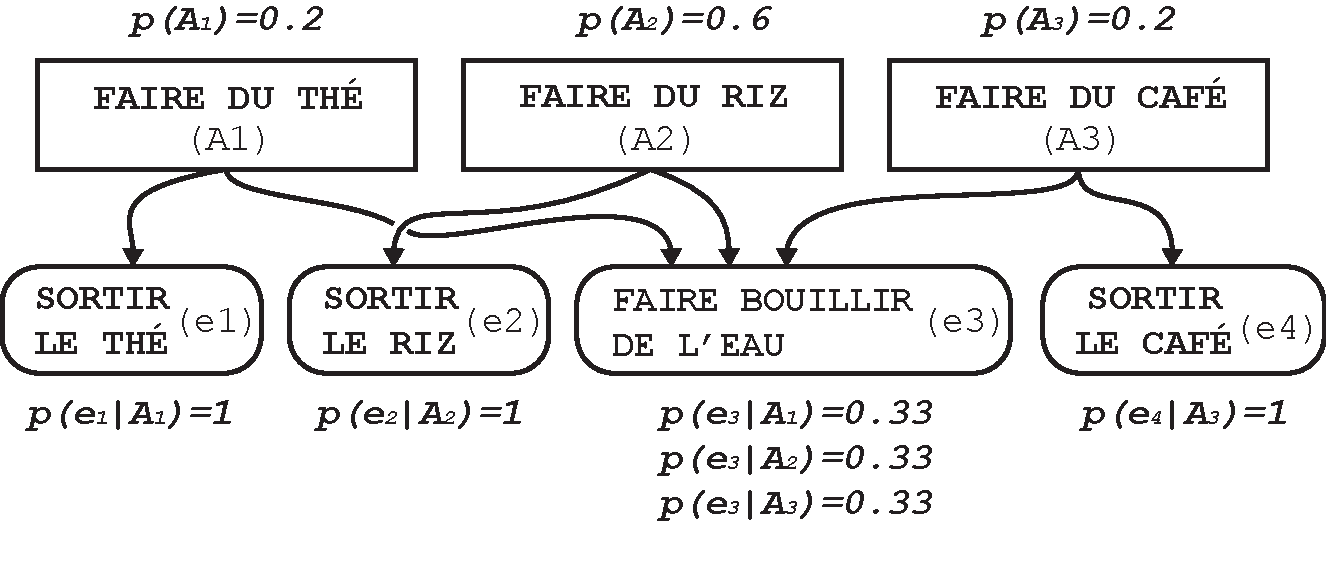
\includegraphics[width=0.8\linewidth]{chapter2/learn_bayes.pdf}
	\caption{Exemple de réseau bayésien naïf.}
	\label{fig:learn_bayes}
\end{figure}

\begin{equation}
	\label{eq:baye_net}
		p(A_i|e_n) = \frac{p(e_n|A_i)\times p(A_i)}{\sum\limits_{j=1}^{J}p(e_j|A_j)\times p(A_j)}
\end{equation}

\noindent où $p(A_i)$ est la probabilité initiale de l'activité $A_i$ et $p(e_n|A_i)$ est la probabilités conditionnelles de l'activité $A_i$ selon l'évènement $e_n$. Grâce aux données fournie par cet exemple, il est donc possible de réaliser l'application numérique suivante à l'aide de l'équation \ref{eq:baye_net} :

\begin{align*}
		p(A_1|e_2)	& = \frac{p(e_2|A_1)\times p(A_1)}{p(e_2|A_1)\times p(A_1) + p(e_2|A_2)\times p(A_2) + p(e_2|A_3)\times p(A_3)} \\[10pt]
					& = \frac{0\times 0.2}{0\times 0.2 + 1\times 0.6 + 0\times 0.2} = 0 \\[20pt]
		p(A_2|e_2)	& = \frac{p(e_2|A_2)\times p(A_2)}{p(e_2|A_1)\times p(A_1) + p(e_2|A_2)\times p(A_2) + p(e_2|A_3)\times p(A_3)} \\[10pt]
					& = \frac{1\times 0.6}{0\times 0.2 + 1\times 0.6 + 0\times 0.2} = 1 \\[20pt]
		p(A_3|e_2)	& = \frac{p(e_2|A_3)\times p(A_3)}{p(e_2|A_1)\times p(A_1) + p(e_2|A_2)\times p(A_2) + p(e_2|A_3)\times p(A_3)} \\[10pt]
					& = \frac{0\times 0.2}{0\times 0.2 + 1\times 0.6 + 0\times 0.2} = 0
\end{align*}

\noindent Finalement, les probabilités sont mises à jour et il apparaît que l’activité \og \textit{faire du riz} \fg ($A_2$) est la seule activité possible puisque celle-ci admet une probabilité de $1$ lorsque l'évènement \og \textit{sortir le riz} \fg ($e_2$) est observé. Le système conclut donc que le résident de l'habitat intelligent est en train de préparer une portion de riz.

Les principaux avantages dans l'utilisation des réseaux bayésiens sont, la simplicité de leur implémentation ainsi que leur performance, tant en termes de taux de reconnaissance dans le cas des activités au sein d'un habitat intelligent, qu'en termes de temps d'exécution et de consommation d'espace mémoire \citep{Friedman1997}. Néanmoins, ceux-ci nécessitent de connaître l'ensemble des activités, des actions et des probabilités conditionnelles qui les relient pour fonctionner ; ce qui constitue un inconvénient majeur, car ces informations ne sont pas toujours disponibles.

Les modèles de Markov cachés (\aclp{HMM} ou \acsp{HMM}) ainsi que les champs aléatoires conditionnels (\aclp{CRF} ou \acsp{CRF}) sont d'autres exemples d'algorithmes statistiques qui ont été utilisés pour la reconnaissance d'activités au sein des habitats intelligents \citep{Oliver2004, Nazerfard2010, VanKasteren2011}. Les \acsp{HMM} peuvent être représentés comme des automates probabilistes à états finis dont l'évolution au cours du temps est entièrement déterminée par une probabilité initiale et des probabilités de transitions entre états. De plus, l'état du système, soit l'activité à reconnaître, n'est pas directement observable, mais caché par un processus d'observation. Autrement dit, au temps $t$, le système qui est dans l'état invisible $q_t$ émet l'observation $O_t$. Ces observations sont, quant à elles, visibles et elles peuvent, par exemple, correspondre à la valeur d'un capteur. Tout comme pour les réseaux bayésiens, les \acsp{HMM} offrent d’excellentes performances de reconnaissance et d’exécution. Néanmoins, la complexité de leur mise en place et de leur compréhension ainsi que la connaissance initiale requise pour leur fonctionnement sont autant de facteurs limitant leur utilisation à la reconnaissance d'un nombre très restreint d’activités.

Par ailleurs, les \acsp{CRF} permettent, quant à eux, de modéliser les dépendances entre un ensemble d’observations réalisées sur une séquence et un ensemble d’étiquettes. En comparaison avec un \acs{HMM}, un \acs{CRF} ne repose pas sur l’hypothèse forte d’indépendance des observations entre elles, conditionnellement aux états associés (les activités). De plus, ils ne combinent pas de probabilités conditionnelles locales, évitant ainsi une estimation biaisée de ces probabilités si trop peu d’exemples étiquetés sont disponibles. Autrement dit, les \acsp{CRF} permettent de limiter le nombre de paramètres initiaux requis dans la mise en place d'un \acs{HMM}, offrant alors une généralisation du modèles de Markov.

\subsubsection{Les arbres de décision}

Les arbres de décision appartiennent à la catégorie des méthodes d'apprentissage supervisées. Comme illustré par la figure \ref{fig:learn_dtree}, la classification des données est faite par une suite de choix logiques représentée sous forme d'un arbre, où chacun de ses n\oe{}uds possède un unique parent excepté le n\oe{}ud racine. Ainsi, les feuilles de l'arbre correspondent aux classes des activités à reconnaître et les n\oe{}uds non terminaux sont des règles de classification qui doivent être vérifiées grâce aux attributs de la donnée qui est testée.

Dans le domaine de la reconnaissance d'activités, les algorithmes d'arbres de décision qui sont les plus fréquemment utilisés sont, \ac{ID3} ainsi que son extension, \texttt{C4.5} \citep{QuinlanRoss1993}. Les principales différences entre ces deux algorithmes sont qu'à l'inverse d'\acs{ID3}, \texttt{C4.5} accepte les variables continues en plus des variables discrètes et ce dernier est également capable de gérer les données manquantes de façon automatique. Enfin, il permet de réduire le risque de sur-apprentissage, qui est très élevé avec l'algorithme \acs{ID3}, grâce à une technique de \textit{pruning} \citep{Bao2004, Ravi2005, Tapia2007}. Ce phénomène intervient lorsque le modèle d'apprentissage est trop similaire aux données d'entraînement et donc plus suffisamment générique pour reconnaître correctement de nouvelles activités. Malgré ces différences, le fonctionnement de ces deux algorithmes reste très similaire. Pour chaque attribut de l'ensemble de données qui n'a pas déjà été traité, son entropie $H$ (\textit{cf. } équation \ref{eq:entropy}) est calculée. Ensuite, l'attribut ayant l'entropie la plus faible est sélectionné et une séparation des données est faite en fonction de celui-ci (\textit{p. ex.} \og \textit{la casserole est sur la cuisinière} \fg ou \og \textit{la casserole n'est pas sur la cuisinière} \fg). Enfin, la structure finale de l'arbre est créée de manière récursive en ne considérant uniquement les attributs qui n'ont jamais été sélectionnés, pour chaque sous-ensemble de données. Ceci vient donc conclure la phase d'entraînement d'un arbre de décision. La phase de reconnaissance, quant à elle, ne nécessite qu'un simple parcours de l'arbre. Ainsi, en reprenant l'exemple de la figure \ref{fig:learn_dtree}\textemdash si les données de l'instance à reconnaître correspondent au positionnement de la casserole sur la cuisinière de l'habitat intelligent, alors l'activité réalisée par le résident est \og \textit{faire du riz} \fg.

\begin{figure}[H]
	\centering
	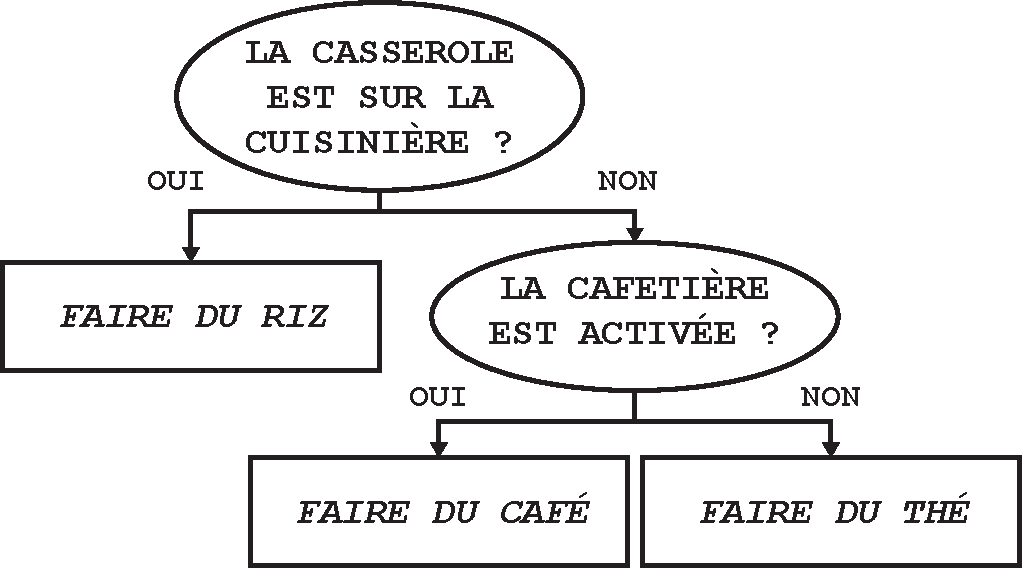
\includegraphics[width=0.7\linewidth]{chapter2/learn_dtree.pdf}
	\caption{Exemple d'un arbre de décision binaire.}
	\label{fig:learn_dtree}
\end{figure}

L'utilisation des arbres de décision offre plusieurs avantages. Dans un premier temps, ceux-ci restent relativement simples à implémenter, mais surtout, ils offrent une très grande facilité de compréhension. De plus, ils ont démontré une excellente performance tant en termes de rapidité d'exécution qu'en termes de taux de reconnaissance \citep{Bao2004}. En revanche, ils se sont révélés beaucoup moins efficaces dans des systèmes impliquant la reconnaissance d'un très grand nombre d'activités parmi lesquelles certaines peuvent se ressembler. De plus, les arbres de décision concèdent deux autres limites importantes qui sont, la nécessité d'avoir un très grand nombre de données pour être entraînés correctement et l'obligation de répéter la phase d'entraînement après chaque ajout d'une nouvelle activité ou après la modification des données d'une activité existante.

\subsubsection{Le \textit{clustering}}

Les méthodes de \textit{clustering} représentent une large partie des algorithmes d'apprentissage non-supervisés \citep{Witten2016}. Le fonctionnement général de toutes les techniques de \textit{clustering} existantes consiste en la division homogène d'un ensemble de données en différents \textit{clusters} qui doivent partager des caractéristiques communes. Les \textit{clusters} sont donc des sous-ensembles des données d'apprentissage. La séparation des données en \textit{clusters} est réalisée, à la fois par minimisation de la distance intra-classe ; c'est-à-dire, la distance entre tous les éléments d'un même \textit{cluster}, ainsi que par la maximisation de la distance inter-classe, qui correspond à la distance entre tous les \textit{clusters}. Ensuite, pour chaque cluster, une donnée représentative lui est attribuée. En fonction de l'algorithme qui est employé, cette dernière peut être déterminée différemment. Dans certains cas, une nouvelle valeur (le barycentre) est calculée à l'aide des données déjà présentes dans le \textit{cluster}. Dans d'autres cas, c'est une donnée existante qui sera élue comme la plus représentative pour chaque \textit{cluster}. Un exemple d'une méthode de \textit{clustering} utilisant le calcul des barycentres est illustré en figure \ref{fig:learn_clustering}.

\begin{figure}[H]
	\centering
	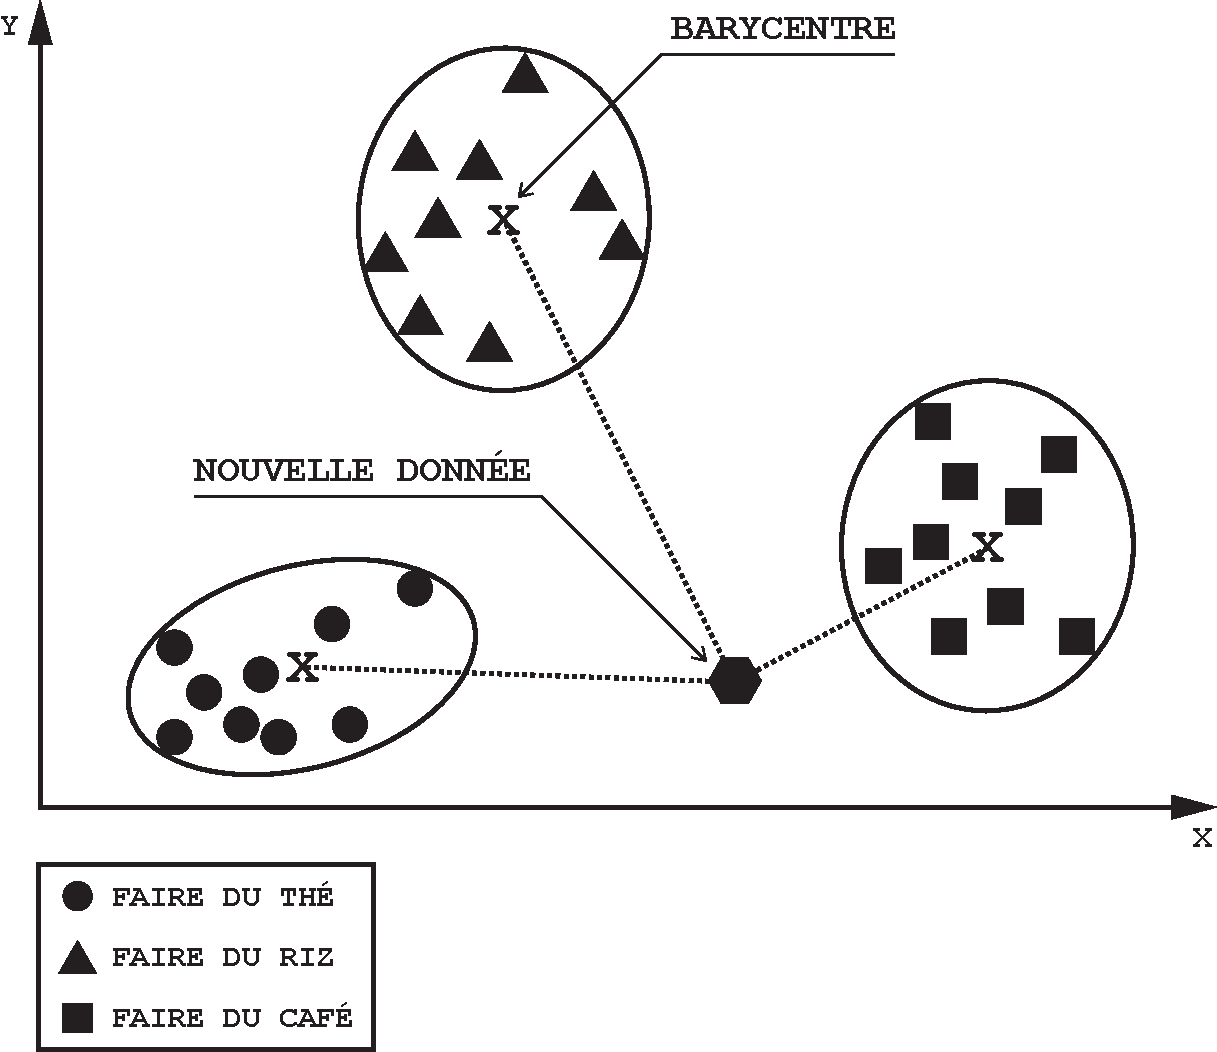
\includegraphics[width=0.6\linewidth]{chapter2/learn_clustering.pdf}
	\caption{Exemple d'un algorithme de \textit{clustering}.}
	\label{fig:learn_clustering}
\end{figure}

L'algorithme de \textit{clustering} le plus utilisé dans le domaine de la reconnaissance d'activités est l'algorithme des $K$-moyennes \citep{Messing2009, Kovashka2010}. Cet algorithme requiert que le nombre total de \textit{clusters} $K$ soit fixé à l'avance. Ainsi, l'algorithme d'apprentissage commence par initialiser les barycentres, où la valeur qui leur est attribuée peut varier en fonction du problème à traiter. En effet, ceux-ci peuvent être initialisés à nul, avec des valeurs purement aléatoires ou encore avec des valeurs prises parmi les données existantes. Lorsque les barycentres sont définis, l'algorithme va, de manière itérative, commencer par calculer la distance de chaque instance de l'ensemble de données par rapport à chacun des $K$ barycentres. Chacune d'elles sera alors associée à son barycentre le plus proche. L'étape suivante consiste à mettre à jour la valeur des barycentres en fonction des \textit{clusters} qui se sont formés. Enfin, ce processus est répété jusqu'à l'obtention d'une convergence, c'est-à-dire, jusqu'à la stabilisation des valeurs des barycentres ; ce qui conduit à l'obtention du modèle d'apprentissage. Comme illustré dans l'exemple de la figure \ref{fig:learn_clustering}, ce modèle d'apprentissage admet trois \textit{clusters}, où chacun d'eux correspond au regroupement des données selon les trois mêmes activités qui sont utilisées depuis le début de ce chapitre. Dès lors, la classification d'une nouvelle instance nécessite de calculer la distance entre cette dernière et tous les barycentres. La plus petite distance obtenue détermine donc à quelle classe d'activité cette nouvelle donnée appartient. Dans cet exemple, la nouvelle donnée correspond donc à l'activité \og \textit{faire du café}\fg. Parmi toutes les mesures de distance qu'il est possible d'utiliser, celles qui sont les plus fréquemment utilisées dans l'algorithme des $K$-moyennes lorsque les données ont $n$ dimensions sont, la distance Euclidienne $D_e$ et la distance de Manhattan $D_m$, respectivement rappelées par les équations \ref{eq:dist_euclidean} et \ref{eq:dist_manhattan} tel que,

\begin{equation}
	\label{eq:dist_euclidean}
	D_e = \sqrt{\sum_{i=1}^{n}(x_i-y_i)^2}
\end{equation}

\begin{equation}
	\label{eq:dist_manhattan}
	D_m = \sum_{i=1}^{n}\left|x_i-y_i\right|
\end{equation}

Bien que le côté non-supervisé de ces méthodes constitue un avantage majeur dans leur utilisation pour reconnaître des activités, elles n'en demeurent pas moins dénuées d'inconvénients. En effet, le processus d'entraînement est souvent coûteux en termes de temps d'exécution et en termes de consommation de la mémoire. De plus, le manque de flexibilité induit par la définition préalable du nombre de \textit{clusters} est un inconvénient majeur pour un système de reconnaissance où le nombre d'activités demeure potentiellement infini. Pour combler ce dernier inconvénient, il est possible de recourir à l'algorithme \ac{DBSCAN}, car son utilisation permet de s'affranchir d'une initialisation manuelle du nombre de clusters. Néanmoins, celui-ci éprouve des difficultés lorsqu'il s'agit de gérer des clusters ayant des densités différentes et ceci est fréquent dans le domaine de la reconnaissance d'activités. \acs{DBSCAN} n'est alors pas toujours le meilleur compromis.

\subsubsection{Les machines à support de vecteurs}

Les machines à support de vecteurs (\ac{SVM}) font partie des techniques d'apprentissage supervisées. L'objectif d'un \acs{SVM} est de créer une séparation des données d'entraînement optimale par le biais d'un hyperplan. De ce fait, l'algorithme va chercher à maximiser la marge, c'est-à-dire, la distance entre l'hyperplan et les données les plus proches de celui-ci. Ces données sont les supports de vecteurs. La figure \ref{fig:learn_svm_a} montre un exemple de machine à support de vecteurs linéaire. En revanche, il est possible que dans certains cas, les données ne soient pas linéairement séparables, c'est-à-dire qu'aucun hyperplan de marge optimale n'existe. Pour pallier cela, il est possible d'utiliser une fonction de noyau (linéaire, quadratique, polynomiale, de base radiale gaussienne, sigmoïde, \textit{etc.}) qui permet alors de convertir des données d'apprentissage en un ensemble de dimension supérieur, où il est possible de créer un hyperplan de marge optimale permettant de séparer les données, tel qu'illustré en figure \ref{fig:learn_svm_b}. Afin d'identifier à quelle classe d'activité la nouvelle donnée appartient, le processus de reconnaissance va simplement calculer de quel côté de l'hyperplan celle-ci se situe. Ainsi, dans le cas de l'exemple proposé en figure \ref{fig:learn_svm_a} la nouvelle donnée est à droite de l'hyperplan, elle est donc identifiée comme l'activité \og \textit{faire du café}\fg.

\begin{figure}[H]
	\centering
	\subfloat[Linéaire]{
		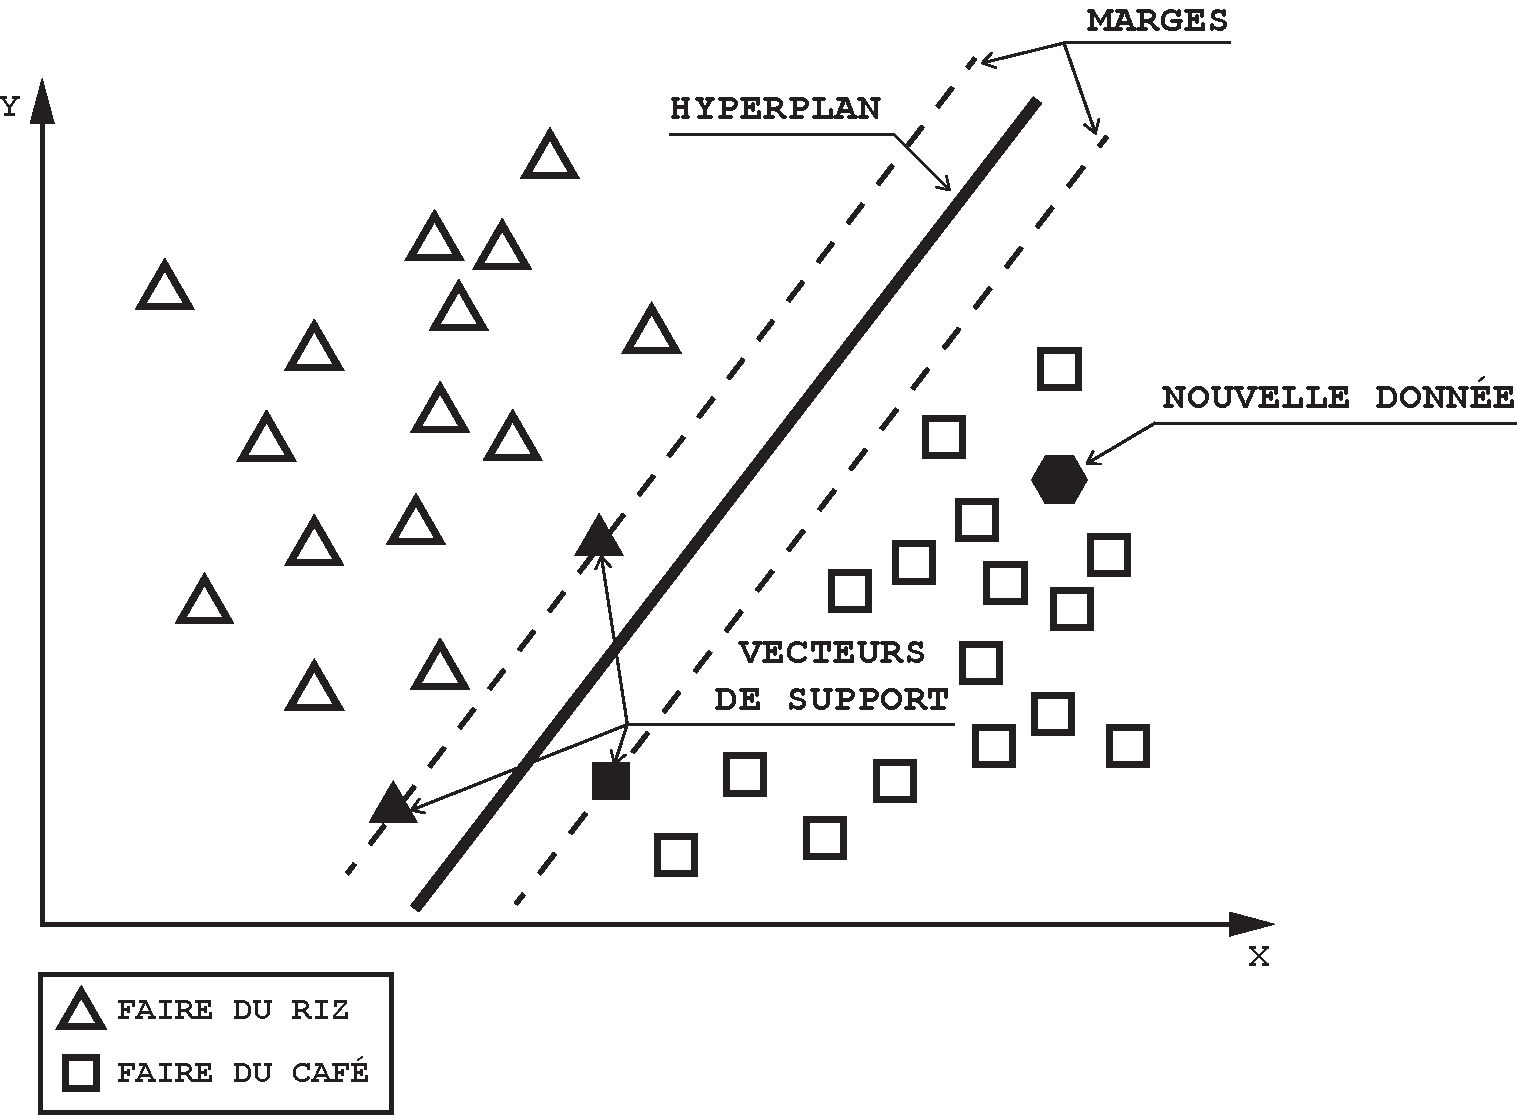
\includegraphics[width=.5\linewidth]{chapter2/learn_svm_a.pdf}
		\label{fig:learn_svm_a}
	}
	\hspace*{\fill}
	\subfloat[Fonction de noyau]{
		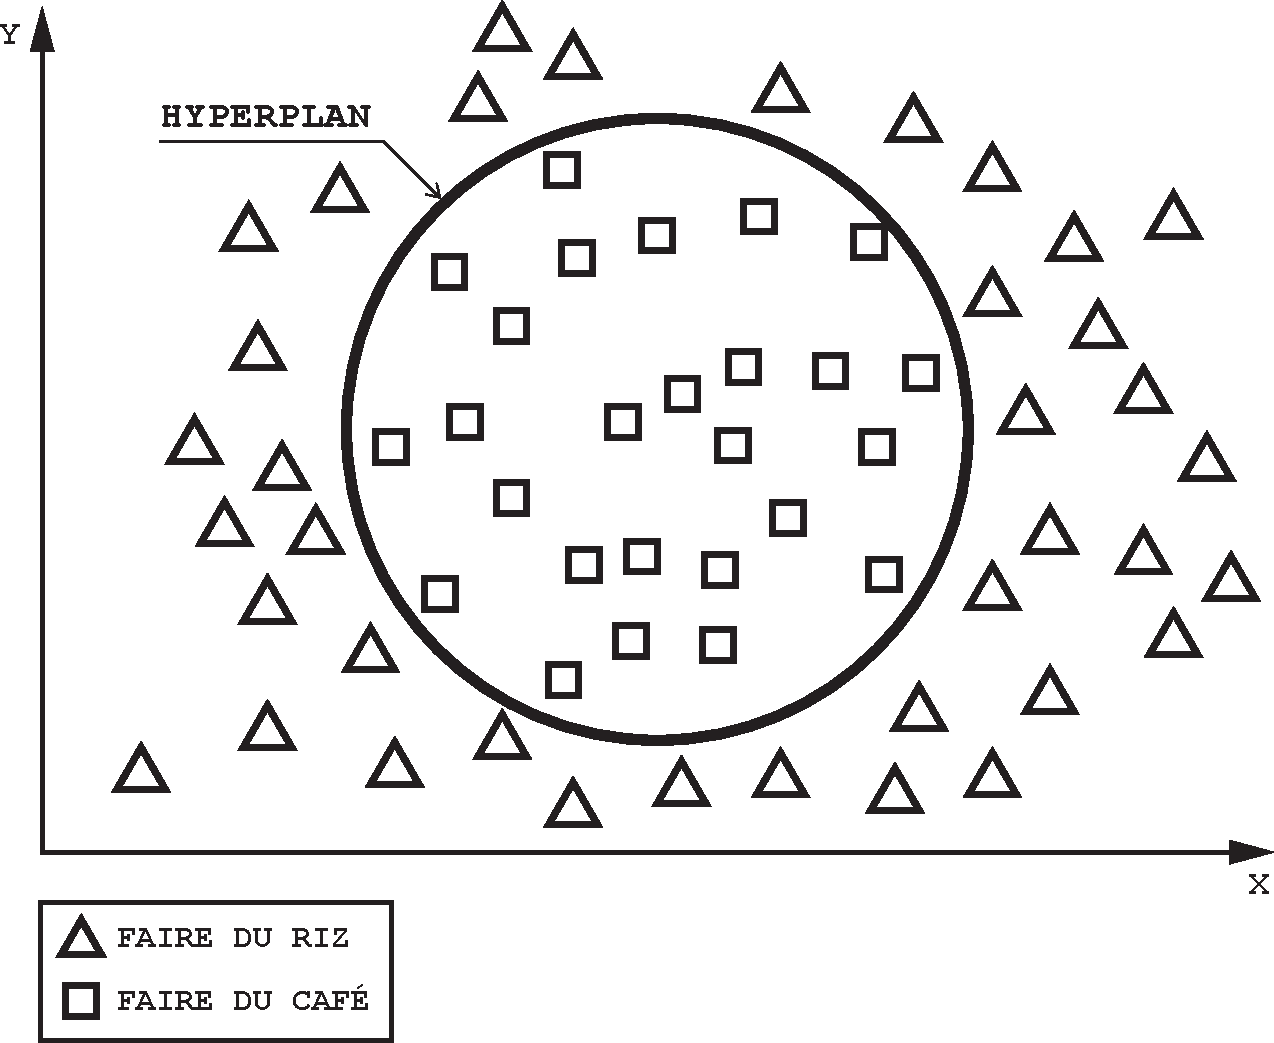
\includegraphics[width=.45\linewidth]{chapter2/learn_svm_b.pdf}
		\label{fig:learn_svm_b}
	}
	\caption{Exemple d'un SVM linéaire ainsi que d'un SVM utilisant une fonction de noyau.}
\end{figure}

Les \acs{SVM} sont souvent considérés comme des boîtes noires, car ils ne permettent pas l'extraction d'un modèle compréhensible, à l'inverse des arbres de décision, par exemple. Néanmoins, ils sont fréquemment utilisés dans le domaine de la reconnaissance d'activités pour plusieurs raisons \citep{He2009, Anguita2012}. La première est qu'ils permettent d'obtenir des taux de reconnaissance très élevés. De plus, le processus de reconnaissance est très efficace en termes de consommation des ressources et peut donc facilement être réalisé sur des systèmes portables. Toutefois, les machines à support de vecteurs ne sont pas adaptées pour traiter un très gros volume de données lors du processus d'apprentissage\textemdash ce dernier impliquant de lourds calculs pour construire le modèle.

\subsubsection{Les réseaux de neurones artificiels}

Les réseaux neurones artificiels (\aclp{ANN} ou \acsp{ANN}) sont des méthodes d’apprentissage qui sont supervisées. Elles visent à imiter la pensée humaine par la modélisation simplifiée des systèmes neuronaux du cerveau de l’Homme et des animaux. Les \acsp{ANN} sont composés de plusieurs neurones connectés entre eux qui s’échangent des signaux \citep{Witten2016}. Chaque neurone est composé d'un nombre $n$ d'entrées synaptiques qui sont chacune associées à un poids ($w$). Celles-ci sont ensuite agglomérées en une seule donnée grâce à un additionneur. Cette valeur est alors passée à une fonction d'activation qui va, pour chacun des neurones, renvoyer un signal de sortie positif ou négatif en fonction d'un certain seuil. Ainsi, pour effectuer un apprentissage supervisé avec les réseaux de neurones, la valeur des poids associés à chacune des synapses doit être modifiée afin que l’erreur entre les sorties du réseau et l'étiquette de la donnée testée soit atténuée. Dès que tous les poids sont mis à jour, la construction du modèle d'apprentissage est terminée et le processus reconnaissance peut commencer. La figure \ref{fig:learn_ann} montre un exemple simplifié d'un perceptron multicouche, l'une des implémentations possibles des \acsp{ANN}, permettant de reconnaître deux activités, \og \textit{faire du riz} \fg et \og \textit{faire du café} \fg. Dans cet exemple, les neurones d'entrée admettent les valeurs des capteurs de l'environnement intelligent et les neurones de sorties correspondent aux activités à reconnaître. Pour simplifier l'exemple, les valeurs de sorties sont exprimées sous la forme de booléens, mais les \acsp{ANN} expriment normalement les sorties sous la forme de probabilités. Par conséquent, c'est la probabilité la plus élevée qui détermine l'étiquette de la donnée testée. Dans ce cas, lorsque le placard est ouvert ; que de l'eau s'écoule du robinet ; que la plaque de cuisson avant-gauche est allumée ; que la casserole est sur la cuisinière et que la cafetière n'est pas allumée, l'activité prédite par cet \acs{ANN} est \og \textit{faire du riz} \fg.

\begin{figure}[H]
	\centering
	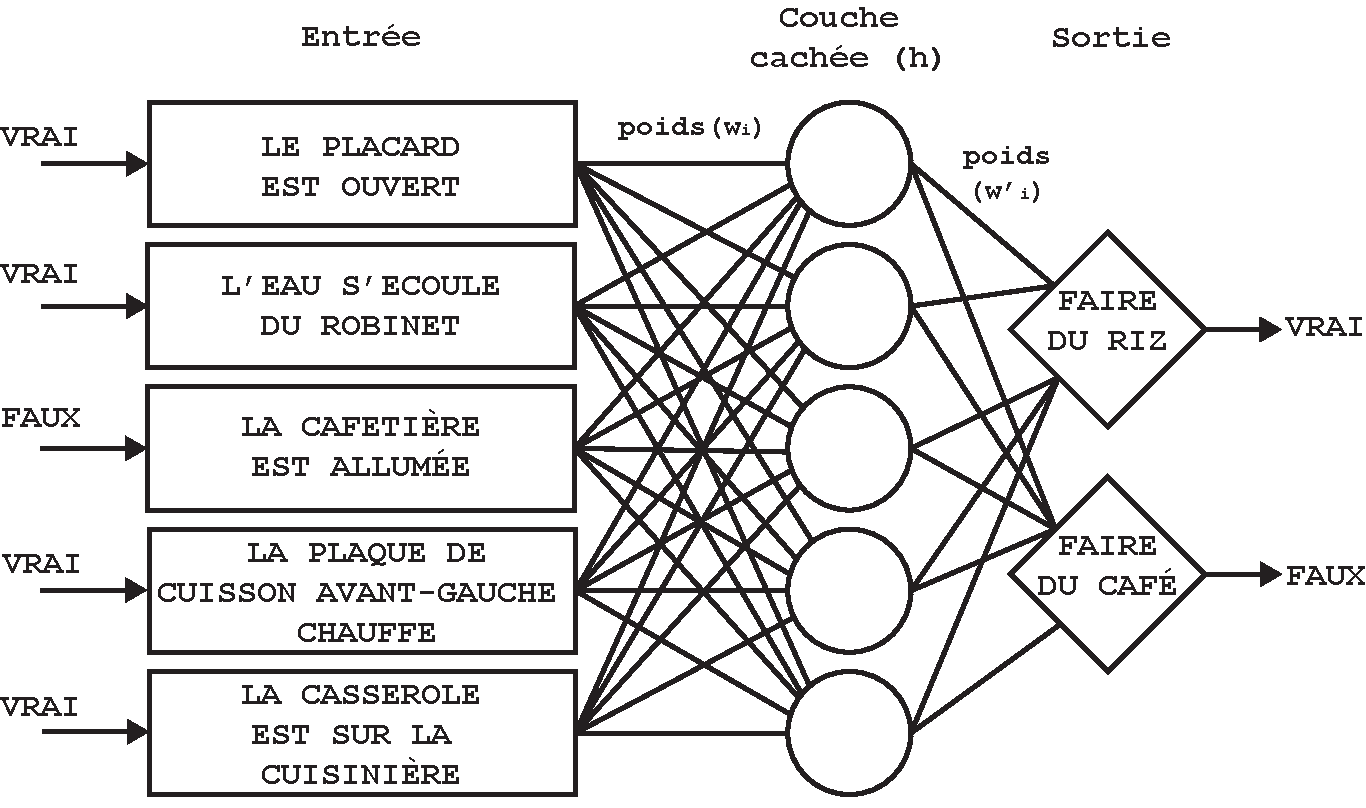
\includegraphics[width=0.8\linewidth]{chapter2/learn_ann.pdf}
	\caption{Exemple de réseau de neurones artificiels.}
	\label{fig:learn_ann}
\end{figure}

De nombreux travaux dans le domaine de la reconnaissance d'activités ont démontré la performance des \acsp{ANN} ainsi que leur robustesse quant à l'exploitation de données fortement bruitées \citep{Parkka2006, Delachaux2013}. Néanmoins, ces techniques nécessitent un temps d'apprentissage considérable pouvant atteindre plusieurs jours. Ceci demeure un inconvénient majeur d'autant plus que ce processus doit être reproduit après chaque ajout d'une nouvelle activité ou après la modification d'une activité déjà existante. De plus, il est très facile, pour un système de reconnaissance basé sur un réseau neural, de tomber dans le sur-apprentissage.

Dans la dernière décennie, l'augmentation exponentielle de la puissance des appareils informatiques a permis de propulser l'utilisation des techniques d'apprentissage profond (deep learning) qui sont des applications particulières des \acsp{ANN} traditionnels qui ont été présenté précédemment. Celles-ci ont démontré leur excellente performance de reconnaissance dans beaucoup de domaines, dont celui de la reconnaissance d'activités \citep{Yang2015, Li2016, Wang2018}. Bien qu'il soit possible que les techniques d'apprentissage profond soient capables de traiter des données brutes directement, c'est-à-dire de se passer de toutes les étapes préliminaires pour la construction du modèle d'apprentissage, elles admettent encore de nombreux inconvénients additionnels à ceux des \acsp{ANN}. En effet, les modèles sont souvent utilisés comme des boîtes noires, car lorsque les résultats obtenus ne sont pas satisfaisants, il est pratiquement impossible d'en expliquer les raisons et surtout de trouver des solutions pour remédier au problème. De plus, ces techniques requièrent un volume conséquent de données pour être entraînées correctement et ainsi, obtenir un modèle générique et réutilisable.

\subsection{La mesure de la performance}

L'étape finale du processus d'apprentissage pour la reconnaissance d'activités consiste en une évaluation de la performance du système. Pour ce faire, il existe de nombreuses métriques qui s'appuient sur l'utilisation d'une matrice de confusion \citep{Fawcett2006}. Cette dernière permet l'identification de la relation qui lie la classe actuelle d'un enregistrement et celle qui est prédite par l'algorithme d'apprentissage. Par exemple, la matrice de confusion retournée par l'un de ces algorithmes dans le cas d'une reconnaissance binaire est donnée par le tableau \ref{tab:conf_mat}. Lorsqu'une instance est positive et qu'elle est prédite comme positive, alors il s'agit d'un vrai positif ($VP$), sinon c'est un faux négatif ($FN$). Dans le cas contraire, si l'instance est négative, et qu'elle est prédite comme positive, alors s'agit d'un vrai négatif ($VN$), sinon c'est un faux positif ($FP$).

\begin{table}[H]
	\begin{center}
		\caption{Matrice de confusion d'un système de reconnaissance binaire.}
		\label{tab:conf_mat}
		\begin{tabular}{llllllllll}
			\cline{3-4}
			& \multicolumn{1}{l|}{} & \multicolumn{2}{c|}{\textbf{classe prédite}} \\ \cline{3-4}
	        & \multicolumn{1}{l|}{} & \multicolumn{1}{c|}{\textbf{oui}} & \multicolumn{1}{c|}{\textbf{non}} \\ \cline{1-4}
			\multicolumn{1}{|c|}{\multirow{2}{*}{\textbf{classe actuelle}}} & \multicolumn{1}{c|}{\textbf{oui}} & \multicolumn{1}{c|}{$VP$} & \multicolumn{1}{c|}{$FN$} \\ \cline{2-4}
			\multicolumn{1}{|c|}{} & \multicolumn{1}{c|}{\textbf{non}} & \multicolumn{1}{c|}{$FP$} & \multicolumn{1}{c|}{$VN$} \\ \cline{1-4}
		\end{tabular}
	\end{center}
\end{table}

Parmi l'ensemble des métriques permettant d'évaluer la performance d'un algorithme d'apprentissage, la mesure de la justesse est la plus fréquemment utilisée, du fait de sa simplicité. Elle permet de déterminer le ratio entre le nombre de prédictions correctement réalisées et le nombre total de cas tel que,

\begin{equation}
	justesse = \frac{VP+VN}{VP+FP+VN+FN}
\end{equation}

Néanmoins, malgré sa popularité, la justesse ne permet pas d'évaluer avec robustesse la qualité des prédictions. En effet, cette dernière ne prend pas en considération les prédictions qui peuvent être faites par chance. Par conséquent, une bonne justesse n'implique pas nécessairement une bonne performance de reconnaissance. C'est le phénomène du \textit{paradoxe de la justesse}. Pour tenir compte de cet effet de bord souvent négligé, d'autres métriques comme la Kappa de Cohen ($k$) ou la $F\mbox{-} mesure$ doivent être calculées \citep{Ben-David2007a}. La première est exprimée par :

\begin{equation}
	\label{eq:kappa}
	k = \frac{P_o - P_e}{1 - P_e}
\end{equation}

\noindent où $P_o$ et $P_e$ sont respectivement, les probabilités observées, c'est-à-dire le taux de succès obtenu par l'algorithme ; et les probabilités espérées, c'est-à-dire le taux de succès hypothétique de l'algorithme. La relation (\ref{eq:f-score}) permet, quant à elle, d'obtenir la $F\mbox{-} mesure$, tel que,

\begin{equation}
	\label{eq:f-score}
	F\mbox{-} mesure = 2 \cdot \frac{pr\acute{e}cision \cdot rappel}{pr\acute{e}cision + rappel}
\end{equation}

\noindent où la $pr\acute{e}cision$ et le $rappel$ sont respectivement donnés par les équations \ref{eq:precision} et \ref{eq:rappel} tel que,

\begin{equation}
	\label{eq:precision}
	pr\acute{e}cision = \frac{VP}{VP+FP}
\end{equation}

\begin{equation}
	\label{eq:rappel}
	rappel = \frac{VP}{VP+FN}
\end{equation}

\section{Conclusion}

Dans un premier temps, ce chapitre s'est intéressé aux habitats intelligents existants qui ont été regroupés en trois catégories. Premièrement, les habitats intelligents académiques \acs{LIARA} et le laboratoire \acs{DOMUS} sont deux architectures qui reposent sur des technologies héritées du milieu industriel. Ces deux habitats, dont le coût total est très dispendieux, ont démontré une faiblesse en termes d'évolutivité et, par conséquent, l'absence d'une quelconque solution pour y intégrer facilement des \textit{wearable devices}. Ensuite, les architectures d'habitats basés composants comme Gator-Tech ou Amiqual4home ont répondu à cette problématique, car elles se sont révélées beaucoup plus flexibles quant à l'intégration de nouveaux composants matériels qu'ils soient de type ambiant ou portable. Néanmoins, la surcharge du serveur central pouvant être occasionnée par un grand nombre de flux de données n'en fait pas pour autant la solution idéale. Enfin, les architectures basées sur un réseau maillé, sont apparues comme les plus avancées en terme de flexibilité pour y intégrer des \textit{wearable devices} malgré le support de la technologie de communication ZigBee uniquement.

Dans sa deuxième partie, ce chapitre a présenté plus en détails l’ensemble des étapes nécessaires pour réaliser le processus d'apprentissage pour reconnaître des activités. Les différentes techniques permettant de raffiner la qualité des données brutes renvoyées par les différemment capteurs et qui constituent la première phase du processus ont été exposés. Ensuite, les algorithmes de d'apprentissage les plus utilisés dans le domaine de la reconnaissance d'activités ont été examinés. Finalement, ce chapitre s'est achevé par la description des différentes méthodes permettant d'évaluer la performance de ces algorithmes et de la qualité intrinsèque de la reconnaissance d'activités.
